\section{Introduction}
\label{sec:intro}

\subsection{Motivation and Preview of Contributions}
\label{sec:intro-motivation} 

We are interested in jointly quantifying uncertainty when predicting several, possibly dependent, continuous outcomes from a shared set of input features.
This problem is motivated by many applications where data-driven decisions depend on several unknown variables rather than on any one of them in isolation. For example, a financial institution may use available customer data to jointly forecast that customer's future credit-line utilization, monthly spending volume, and credit score. In this and many other contexts, decision quality hinges on the joint reliability of all predicted values, and an output that is incorrect in even one dimension could lead to adverse consequences.

Conformal prediction is a popular and broadly applicable framework for uncertainty quantification in predictive settings \citep{vovk2005algorithmic, angelopoulos2023conformal}. It derives its main strengths from the ability to augment the output of any machine-learning model with {\em prediction sets} equipped with finite-sample guarantees, without relying on strong assumptions on the data distribution. Its sole assumption is the availability of labeled data that are {\em exchangeable} with the test point of interest, a weaker requirement than the standard assumption of i.i.d.~sampling. For a {\em univariate} setting, where the goal is to predict a single continuous-valued outcome, there now exist several well-established conformal prediction methods that produce valid, computationally fast, and easy-to-interpret prediction intervals \citep{lei2018distribution, romano2019conformalized, sesia2021conformal}.

Extending conformal prediction to the {\em multivariate} setting is a non-trivial problem that has attracted considerable recent interest, spurring a variety of solutions \citep{dheur2025unified}. The fundamental challenge is to aggregate a vector of generalized residuals—whose components may differ substantially in scale and variability—into a scalar-valued {\em non-conformity score} leading to {\em prediction sets} that should satisfy four key desiderata: (i) finite-sample coverage, (ii) informativeness or tightness, (iii) computational tractability, and (iv) interpretability.
Interpretability can take different meanings depending on the application, and in some settings it is consistent with prediction sets having complex shapes. Nevertheless, in many practical scenarios, hyper-rectangular prediction sets—or, equivalently, jointly valid prediction intervals—provide the most natural and transparent way to convey uncertainty to practitioners. This paper focuses on such settings.

Existing methods achieve only a subset of these desiderata. The simplest approach to obtain hyper-rectangular prediction sets is to apply univariate conformal prediction to each output and then take the Cartesian product of the resulting intervals \citep{neeven2018conformal}; however, a conservative Bonferroni adjustment to the marginal miscoverage levels is needed to guarantee joint coverage; see Algorithm~\ref{alg:bonferroni} in Appendix~\ref{app:algorithms}. This strategy is very easy to implement, but the Bonferroni correction is often too conservative to be practically satisfactory, as it adopts a worst-case view of the dependence structure across output dimensions.
By contrast, we aim to achieve valid coverage with joint prediction intervals that are as tight as possible; see Figure~\ref{fig:joint-prediction} for a sketch of this goal.

\begin{figure}[!htb]
    \centering
    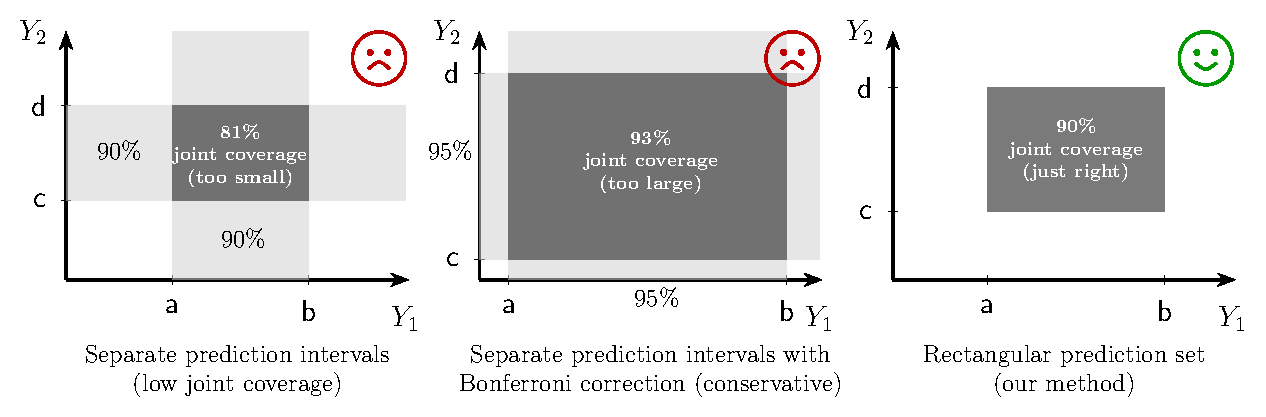
\includegraphics[width = 0.9\textwidth]{figures/joint_prediction.pdf}
\caption{Two-dimensional toy example depicting graphically the main objective of this work: constructing \emph{informative} and \emph{interpretable} hyper-rectangular conformal prediction sets for multivariate outcomes. 
Left: univariate approaches can produce marginal prediction intervals for each output separately, which do not guarantee joint coverage. 
Center: a Bonferroni correction can easily restore valid joint coverage, at the cost of being overly conservative. 
Right: our goal is to efficiently construct hyper-rectangular prediction sets that are easy to interpret and retain valid coverage; doing so involves technical challenges.}
    \label{fig:joint-prediction}
\end{figure}

A second class of methods reduces multivariate residuals to scalar-valued non-conformity scores, for example by applying an $\ell_2$ or $\ell_\infty$ norm, applies univariate conformal calibration to these scores, and maps the resulting score threshold back into the original output space; see Algorithm~\ref{alg:unscaled} in Appendix~\ref{app:algorithms}. While computationally efficient and able to produce hyper-rectangular prediction sets when using the $\ell_\infty$ norm, these approaches can be dominated by the noisiest dimension, leading to prediction sets that are unnecessarily wide along low-uncertainty directions.

More sophisticated approaches have been developed to directly minimize the volume of the resulting prediction sets, for example using optimal transport, learned embeddings, copulas, or generative models to describe the dependence structure across residual dimensions. However, these methods aim to solve a problem that is different from that considered in this paper, since they are explicitly designed to produce non-rectangular prediction sets. Moreover, they often introduce substantial computational overhead and require additional independent training data to provide finite-sample guarantees.

In this paper we focus on targeting what we believe is the core difficulty in many applications: the mismatch in the {\em marginal} scale and variability of residuals across output dimensions. 
To address this challenge, we develop a method based on transductive coordinate-wise residual standardization. This restores comparability across coordinates and enables the construction of tight hyper-rectangular prediction sets that guarantee finite-sample coverage, without necessitating additional training data or prohibitive computational overhead. Remarkably, our method does {\em not} need to explicitly model residual dependencies across different dimensions, unlike existing approaches focusing on non-rectangular prediction sets.

Making this idea operational requires overcoming several hurdles, which we resolve through a sequence of increasingly practical steps. We begin by formulating an ideal oracle procedure that assumes access to the test point’s true outcome vector and uses this information to standardize the multi-dimensional residuals in the calibration set without violating the exchangeability conditions that are necessary to guarantee finite-sample coverage. Although clearly impractical, this oracle is valuable to guide the design of our practical method.
Inspired by the oracle procedure, we introduce two increasingly sophisticated data-driven approaches. The first provides a more conservative approximation of the oracle, whereas the second achieves greater statistical efficiency by building on top of the first. Through extensive numerical experiments, we demonstrate that this progression of ideas culminates in a practical method producing prediction sets satisfying all our desiderata.


\subsection{Related Work}
\label{sec:related-work}

Extending conformal prediction to multivariate outcomes has attracted substantial attention in recent years, leading to the development of a wide range of alternative methods.

A prominent line of work seeks minimum-volume prediction sets with flexible geometries by modeling dependence across output dimensions.
This includes copula-based approaches \citep{messoudi2021copula, pmlr-v258-park25c, sun2024copula}, non-parametric density estimation methods \citep{sadinle2016least,izbicki2022cdsplit,wang2023pcp, dheur2025unified}, parametric density estimation methods \citep{johnstone2021conformal,braun2025minimum,braun2025multivariate,tumu2024templates}, optimal-transport techniques \citep{thurin2025otcp, klein2025multivariate}, and flow-based generative models \citep{colombo2024normalizing, lee2025flow, fang2025contra}. While these approaches can produce smaller prediction sets than our method, the resulting sets often have complex shapes that are more difficult to interpret. Moreover, these approaches require additional model training on independent data to provide finite-sample guarantees, and many also involve substantial computational overhead.

To the best of our knowledge, the idea of directly addressing heterogeneity across output dimensions via marginal residual rescaling remains relatively under-explored. \citet{baheri2025multiscale} pursue a related idea, but rely on a conservative Bonferroni-type correction. {\color{blue}The approach of \citet{sampson2024conformal} is more closely related to ours, but their method requires a base region of predictions, which one would need to estimate through an additional independent dataset if not provided directly through model estimation; avoiding this requirement is the main technical challenge addressed in our paper. As we show empirically, the methods of \citet{sampson2024conformal} are often considerably less efficient than ours—particularly in small-sample regimes—resulting in less stable and less informative prediction sets.}

Our solution can be viewed as implementing a special instance of transductive, or full, conformal prediction \citep{vovk2005algorithmic,vovk2013transductive}. In contrast to the more commonly used split conformal methods, full conformal prediction repeatedly incorporates the test point, augmented with different candidate labels, directly into a learning algorithm. Although this strategy is computationally prohibitive in general, especially for continuous-valued numerical outcomes and complex algorithms, it can be implemented efficiently in some cases by exploiting structural properties of the underlying predictive model. Accordingly, our paper relates to a broader literature on making full conformal inference computationally practical in special cases, including approaches tailored to sparse generalized linear models \citep{lei2019fast,guha2023conformalization} and methods that leverage stability or other forms of structure in the predictive model \citep{ndiaye2019computing, abad2022approximating, martinez2023approximating, li2024generalized}. Unlike those works, which focus primarily on accelerating model refitting, we assume a fixed, pre-trained model and instead aim to improve efficiency by avoiding calibration data splitting while explicitly standardizing residuals across output dimensions. Both the problem setting and the proposed methodology are therefore novel.

More broadly, our approach is also related to recent conformal methods that reuse calibration data for different purposes, such as enabling early stopping to control overfitting when training deep learning models \citep{liang2023conformal} and leveraging data-adaptive grouping to improve conditional coverage \citep{zhou2024conformal, zhang2024posterior}. In contrast to these works, our focus is on addressing heterogeneity across targets in multivariate regression while obtaining interpretable, rectangular prediction sets.


\subsection{Outline}

This paper is organized as follows.
Section~\ref{sec:preliminaries} introduces notation, formal problem statement, and the required assumptions, along with a description of an ideal population oracle approach that has access to population-level information.
Section~\ref{sec:methods} presents our methodology, starting with a transductive oracle that knows the unobserved test outcome, followed by the general construction of our method along with its computable implementations.
Section~\ref{sec:experiments} validates our method empirically and compares its performance to that of existing approaches using both simulated and real data.
Section~\ref{sec:discussion} discusses some limitations and possible directions for future research.
The appendices contain the remaining mathematical proofs, additional algorithmic details, and further numerical results.

\clearpage

\section{Problem Setup and Motivating Constructions}
\label{sec:preliminaries}

In this section, we present the formal mathematical formulation of our problem of interest along with the motivation of our solution and discuss all the necessary background to understand our method to be introduced in Section~\ref{sec:methods}.

\paragraph{Notation}

For any $m\in\mathbb N$, we use $[m]:=\{1,\ldots,m\}$ to denote the set of $m$ indices.
For any $m\in\mathbb N$, $\alpha\in(0,1)$, and $(v_1,\ldots,v_m)\in\mathbb R^m$, we use $\hat Q_{1-\alpha}(v_1,\ldots,v_m)$ to denote the $\lceil(1-\alpha)(m+1)\rceil$-th smallest value of the augmented list $(v_1,\ldots,v_m,+\infty)$, counting repeated values separately. We write $\overline{\R}:=\R\cup\{-\infty,+\infty\}$.

\subsection{Problem Setup}

We consider a multi-output (multivariate) regression setting where the goal is to predict a vector $\mathbf Y=(Y_1,\ldots,Y_d)$ of $d$ real-valued outputs given input features $\mathbf X\in\mathcal X$.

Assume that $(\mathbf X^1,\mathbf Y^1),\ldots,(\mathbf X^{n+1},\mathbf Y^{n+1})$, with $n\geq2$, are jointly exchangeable, with common marginal distribution $P_{X,Y}$. This includes the case where the observations are drawn i.i.d.\ from an arbitrary distribution $P_{X,Y}$. We observe the calibration data $\dataset_{\mathrm{cal}}=\{(\mathbf X^i,\mathbf Y^i)\}_{i=1}^n$ and the test input (covariate) $\mathbf X^{n+1}$, while the corresponding outcome $\mathbf Y^{n+1}$ remains unobserved and to be predicted. Our paper focus on the following two inferential targets of $\mathbf Y^{n+1}$.

\paragraph{Marginal Coverage}

Using all of the observed data, the task is to construct a reasonably tight prediction set $\hat C(\mathbf X^{n+1})\subseteq\mathbb R^d$ that contains the unknown output $\mathbf Y^{n+1}$ with high probability, guaranteeing \emph{marginal coverage}:
\begin{equation}
\mathbb P\!\left[\mathbf Y^{n+1}\in\hat C(\mathbf X^{n+1})\right]\geq1-\alpha,
\label{eq:joint-coverage}
\end{equation}
where $\alpha\in(0,1)$ is the user-specified miscoverage level.
The term ``marginal coverage'' means that the guarantee in~\eqref{eq:joint-coverage} averages over the joint randomness of the calibration samples $\dataset_{\mathrm{cal}}$ and the test point $(\mathbf X^{n+1},\mathbf Y^{n+1})$.

Stronger notions of guarantees, such as coverage conditional on a certain realization of $\mathbf X^{n+1}$, are generally unattainable in finite samples with finite, informative prediction sets and without more restrictive assumptions on the distribution \citep{foygel2021limits}. Methods that approximate conditional coverage \citep{Romano2020With,gibbs2025conformal} may be combined with our approach. Investigating such combinations is an interesting direction for future work but is beyond the scope of this paper.

\paragraph{Interpretability}

In addition to coverage, we seek prediction sets with a simple, interpretable geometry. For the standard residual choices considered in the next section, our method produces \emph{hyper-rectangular} prediction sets, or Cartesian products of univariate prediction intervals:
\begin{equation}\label{eq:rectangle}
\hat C(\mathbf X^{n+1})
=
\bigtimes_{j=1}^d
\left(
\left[L_j(\mathbf X^{n+1}),U_j(\mathbf X^{n+1})\right]
\cap\R
\right),
\end{equation}
where $[L_j(\mathbf X^{n+1}),U_j(\mathbf X^{n+1})]$ denotes the coordinate-wise interval for the $j$th output. We intersect each interval with $\R$ for mathematical completeness since the coordinatewise bounds are allowed to be infinite.

Prediction sets of the form~\eqref{eq:rectangle} provide a separate interval to quantify the uncertainty of each output, making them easy to interpret in the context of multi-output prediction: they tell us exactly which component misses the true response when a prediction set fails, as displayed in Table~\ref{tab:toy}.
For such sets, the marginal coverage requirement in~\eqref{eq:joint-coverage} is equivalent to
\[
\mathbb P\left[
Y_j^{n+1}\in[L_j(\mathbf X^{n+1}),U_j(\mathbf X^{n+1})]
\text{ for all }j\in[d]
\right]\geq1-\alpha.
\]
Thus, although the coverage guarantee is marginal over the calibration and test data, it is simultaneous across all $d$ output coordinates.

In the following subsections, we will discuss how the coverage and interpretability requirements could be achieved in the context of split conformal prediction.


\subsection{Coordinate-Wise Generalized Residuals}
\label{sec:residuals}

In the univariate case, split conformal prediction uses a common choice of nonconformity score to measure disagreement between a candidate output and a pre-trained model's prediction and build prediction intervals through exchangeable calibration of the scores. Our construction extends this idea to multivariate outputs by defining a generalized residual for each output coordinate. These residuals are then calibrated jointly to obtain a prediction set for the full output vector.

We start by assuming access to a \emph{pre-trained} joint predictive model $\hat{\mathbf f}=(\hat f_1,\ldots,\hat f_d)$, fitted on a training dataset independent of both the calibration set $\dataset_{\mathrm{cal}}$ and the test point.
We treat this model as a black box. The only requirement is that it allows us to compute a measurable coordinate-wise \emph{generalized residual} map $\mathbf E:\mathcal X\times\mathbb R^d\to\mathbb R^d$ of the form
\[
\mathbf E(\mathbf X,\mathbf Y)
=
\bigl(E_1(\mathbf X,Y_1),\ldots,E_d(\mathbf X,Y_d)\bigr).
\]

Each component of the residual map assesses agreement between an output and the corresponding fitted prediction, with larger values indicating greater disagreement. Most residual maps have a coordinatewise lower bound at each input $\mathbf x\in\mathcal X$ to represent the scenario of perfect prediction, and some may have a coordinatewise upper bound depending on the data. We denote these two bounds here coordinatewise by $[a_j(\mathbf x),b_j(\mathbf x)]$, where
\[
a_j(\mathbf x)
=
\inf_{y_j\in\R}E_j(\mathbf x,y_j),
\qquad
b_j(\mathbf x)
=
\sup_{y_j\in\R}E_j(\mathbf x,y_j),
\qquad
\mathbf x\in\mathcal X.
\]
In most cases, $b_j(\mathbf X^{n+1})\equiv+\infty$ because the disagreement can be arbitrarily large for bad predictions. Thus, we will use $+\infty$ as a coordinatewise upper bound throughout this paper.

We supply two standard choices of residuals in the context of multivariate predictions here along with their coordinatewise lower bounds and upper bounds when no additional information is given from the data:
\begin{enumerate}
    \item \emph{Absolute residuals}: for a model $\hat f_j$ providing a point prediction of $Y_j$, such as an estimate of the conditional mean $\mathbb E[Y_j\mid\mathbf X]$, a standard choice is
    \[
    E_j(\mathbf X,Y_j)
    =
    \lvert Y_j-\hat f_j(\mathbf X)\rvert
    \]
    \citep{lei2018distribution}; its coordinatewise lower bounds and upper bounds are simply $a_j(\mathbf X^{n+1})\equiv0$ and $b_j(\mathbf X^{n+1})\equiv+\infty$ for all $j\in[d]$.

    \item \emph{Quantile residuals}: for models that estimate conditional quantiles, as in conformalized quantile regression \citep{romano2019conformalized}, a natural choice is
    \[
    E_j(\mathbf X,Y_j)
    =
    \max\bigl\{
    \hat f_j^{\mathrm{lo}}(\mathbf X)-Y_j,\;
    Y_j-\hat f_j^{\mathrm{hi}}(\mathbf X)
    \bigr\},
    \]
    where $\hat f_j=(\hat f_j^{\mathrm{lo}},\hat f_j^{\mathrm{hi}})$ with $\hat f_j^{\mathrm{lo}}(\mathbf X)\leq\hat f_j^{\mathrm{hi}}(\mathbf X)$ denotes the pair of estimated lower and upper conditional quantiles of $Y_j\mid\mathbf X$, for example at levels $\alpha/2$ and $1-\alpha/2$.

    This residual measures the signed distance of $Y_j$ to the nearest boundary of the interval $[\hat f_j^{\mathrm{lo}}(\mathbf X),\hat f_j^{\mathrm{hi}}(\mathbf X)]$: positive values indicate that $Y_j$ falls outside the interval, negative values indicate that it lies strictly inside, and zero indicates that it lies on the boundary. Hence, the coordinatewise lower bounds of this residual are actually input dependent, i.e.,
    \[
    a_j(\mathbf X^{n+1})
    =
    -\frac12\left(
    \hat f_j^{\mathrm{hi}}(\mathbf X^{n+1})
    -
    \hat f_j^{\mathrm{lo}}(\mathbf X^{n+1})
    \right),
    \]
    and its coordinatewise upper bounds are still $b_j(\mathbf X^{n+1})\equiv+\infty$.
\end{enumerate}

Applying the generalized residual map to the calibration data gives $\mathbf E^i=\mathbf E(\mathbf X^i,\mathbf Y^i)=(E_1^i,\ldots,E_d^i)$ for all $i\in[n]$.
We reserve $\mathbf E^{n+1}=\mathbf E(\mathbf X^{n+1},\mathbf Y^{n+1})$ for the unobserved residual vector of the test point.
Because the same independently fitted residual map is applied to every observation, the calibration and test residual vectors remain exchangeable.

This exchangeability preservation alone is sufficient for the basic conformal coverage guarantee below. Additional regularity conditions used in our method will be introduced in Section~\ref{sec:pop-oracle}.

\subsection{Conformal Calibration with Marginal Coverage}
\label{sec:calibration}

Given the calibration residuals $\mathbf E^1,\ldots,\mathbf E^n$, we construct a prediction set by accepting candidate outputs whose residuals fall below an upper bound in each coordinate:
\begin{equation}
\hat C(\mathbf X^{n+1})
=
\left\{
\mathbf y\in\mathbb R^d:
a_j(\mathbf X^{n+1})
\leq E_j(\mathbf X^{n+1},y_j)\leq W_j
\text{ for all }j\in[d]
\right\}.
\label{eq:joint-prediction}
\end{equation}
Here, $W_1,\ldots,W_d$ are suitable data-dependent upper bounds, possibly infinite, chosen to satisfy
\begin{equation}
\mathbb P\!\left[
E_j(\mathbf X^{n+1},Y_j^{n+1})\leq W_j
\text{ for all }j\in[d]
\right]\geq1-\alpha.
\label{eq:coordinate-threshold}
\end{equation}
By construction, this condition is equivalent to the marginal coverage requirement in~\eqref{eq:joint-coverage}. If the residual map is fixed, increasing the thresholds coordinatewise can only enlarge the prediction set, giving us a route to replace any unknown thresholds by computable ones.

For the two common choices of residuals introduced above, each coordinate of the prediction set in~\eqref{eq:joint-prediction} becomes a prediction interval: (i) $\left[\hat f_j(\mathbf X^{n+1})-W_j,\hat f_j(\mathbf X^{n+1})+W_j\right]$ for absolute residuals and (ii)
$\left[
\hat f_j^{\mathrm{lo}}(\mathbf X^{n+1})-W_j,\;
\hat f_j^{\mathrm{hi}}(\mathbf X^{n+1})+W_j
\right]$
for quantile residuals, hence indicating the final hyper-rectangular geometry.

{\color{brown}
It is worth mentioning that quantile residuals could lead to empty prediction sets if
\[
W_j<
-\frac12\left(
\hat f_j^{\mathrm{hi}}(\mathbf X^{n+1})
-
\hat f_j^{\mathrm{lo}}(\mathbf X^{n+1})
\right)
\]
for some $j\in[d]$, although marginal coverage ensures that the probability of an empty prediction set is at most $\alpha$. \citet{Sesia_2020} presents several modifications to quantile residuals to prevent the existence of empty sets, but we stick to the common choice presented above in this paper.
}

Also, for a general residual map, our intended construction in~\eqref{eq:joint-prediction} need not be hyper-rectangular in the outcome space. Due to the variability of tasks in reality, it might be inefective to enforce a hyper-rectangular geometry in the outcome space for every possible residual map. Our construction in~\eqref{eq:joint-prediction} instead describes the prediction set through coordinatewise bounds on the residuals, therefore ensuring the corresponding acceptance region is hyper-rectangular in the residual space and offering a sense of interpretability.

Finding suitable (informative) thresholds $W_1,\ldots,W_d$ satisfying~\eqref{eq:coordinate-threshold} is also non-trivial.
A naive way to achieve~\eqref{eq:coordinate-threshold} is to set $W_j=\hat Q_{1-\alpha/d}(E_j^1,\ldots,E_j^n)$, which is equivalent to applying univariate conformal prediction separately across all $d$ outcomes, with a Bonferroni correction ($\alpha/d$ replacing $\alpha$).
This typically leads to very conservative prediction sets because it takes an overly pessimistic worst-case view of possible dependencies across outcomes.

In this paper, we pursue a more efficient approach, beginning with induced {\em scalar} non-conformity scores $S^i=\Phi(\mathbf E^i)\in\mathbb R$ for all $i\in[n]$, computed using a measurable scalarization map $\Phi:\mathbb R^d\to\mathbb R$ whose form will be discussed below. We similarly write $S^{n+1}=\Phi(\mathbf E^{n+1})$ for the unobserved test score.
Then, the prediction set is constructed as
\begin{equation}
\hat C(\mathbf X^{n+1})
=
\left\{
\mathbf y\in\R^d:
\Phi(\mathbf E(\mathbf X^{n+1},\mathbf y))
\leq\hat Q_{1-\alpha}(S^1,\ldots,S^n)
\right\}.
\label{eq:joint-prediction-scalar}
\end{equation}
If we make sure $\Phi$ comes from a function class where, for each scalarization map $\Phi$, there exists a threshold map $g=(g_1,\ldots,g_d):\overline{\R}\to\overline{\R}^d$ such that
\[
\Phi(\mathbf e)\leq c
\iff
e_j\leq g_j(c)\text{ for all }j\in[d],
\qquad
\mathbf e\in\R^d,\quad c\in\overline{\R},
\]
then we can recover the form of~\eqref{eq:joint-prediction} using thresholds $W_j=g_j(\hat Q_{1-\alpha}(S^1,\ldots,S^n))$. We focus on transformations with this property, including the standardized maximum introduced below, but the coverage guarantee holds for other choices of $\Phi$, as demonstrated by the following theorem.

\begin{theorem}[Generalized Marginal Coverage]
\label{thm:fixed-transformation-coverage}
Assume $(\mathbf E^1,\ldots,\mathbf E^{n+1})$ are exchangeable, with $\mathbf E^i=\mathbf E(\mathbf X^i,\mathbf Y^i)\in\mathbb R^d$ for all $i\in[n+1]$.
Let $\Phi:\mathbb R^d\to\mathbb R$ be any fixed measurable function, and write $S^i=\Phi(\mathbf E^i)$.
Then the prediction set in~\eqref{eq:joint-prediction-scalar} satisfies
$\mathbb P\!\left[
\mathbf Y^{n+1}\in\hat C(\mathbf X^{n+1})
\right]\geq1-\alpha.$
Moreover, if $S^1,\ldots,S^{n+1}$ are almost surely distinct, then
$\mathbb P\!\left[
\mathbf Y^{n+1}\in\hat C(\mathbf X^{n+1})
\right]\leq1-\alpha+\frac1{n+1}.$
The same result holds for a random $\Phi$ if $(S^1,\ldots,S^{n+1})$ are exchangeable conditional on $\Phi$.
\end{theorem}

Although Theorem~\ref{thm:fixed-transformation-coverage} establishes marginal coverage overall, the guarantee alone does not yield similar coverage probabilities across different outputs.
Depending on the residual distribution and the choice of $\Phi$, some intervals may be much wider than necessary, making the resulting uncertainty estimates less informative (see Figure~\ref{fig:body-abs-coordinate-bars} for an example).

Several recent works consider norm-based scalarizations, such as $\Phi(\mathbf e)=\|\mathbf e\|_p$ for $1\leq p\leq\infty$ \citep{johnstone2022exact}.
Although conceptually and computationally simple, these can be dominated by a residual coordinate with a much larger scale than the others, leading to unnecessarily large acceptance regions in the remaining coordinates.

To obtain tighter prediction sets, recent works have proposed learning a transformation of the residuals before applying a norm-based scalarization, for example through optimal transport \citep{thurin2025otcp,klein2025multivariate}.
However, estimating these transport maps requires additional data splitting of the calibration dataset to preserve exchangeability and substantial computation, and the resulting prediction sets can have complicated geometries (even in the residual space).

We pursue a route similar to these two approaches, but
instead of learning a complicated transformation on the observed data, we propose a simple and interpretable transformation that standardizes the residuals coordinatewise and takes their maximum across coordinates without taking absolute values. Our standardization also uses estimates from the observed data, but in a way that retains finite-sample marginal coverage and avoids additional data splitting.
This construction also yields rectangular prediction sets for the standard residual choices above and aims to avoid unnecessarily conservative intervals in some output dimensions.

\subsection{A Population-Standardized Oracle}
\label{sec:pop-oracle}

To motivate our method, we first consider an oracle construction that has access to the coordinate-wise population means and standard deviations of the residuals.
Although unavailable in practice, this construction illustrates how coordinate-wise standardization can mitigate heterogeneity in residual scales while preserving coverage and, for standard residual choices, rectangular interpretability.

Consider prediction sets of the form in~\eqref{eq:joint-prediction-scalar}, obtained by transforming the vector-valued residuals $\mathbf E^i$ using the following family of scalarization maps:

\begin{equation}
\Phi(\mathbf t;\boldsymbol\beta,\boldsymbol\theta)
:=\max_{1\leq j\leq d}\frac{t_j-\beta_j}{\theta_j},
\qquad\mathbf t\in\mathbb R^d,
\label{eq:residual-transformation}
\end{equation}
where $\boldsymbol\beta=(\beta_1,\ldots,\beta_d)^\top$ and $\boldsymbol\theta=(\theta_1,\ldots,\theta_d)^\top$, with $\theta_j>0$ for all $j\in[d]$, are vectors of location and scale parameters, respectively.
This transformation certainly has the coordinate-wise representation, discussed earlier in Section~\ref{sec:calibration}:
\[
\Phi(\mathbf t;\boldsymbol\beta,\boldsymbol\theta)\leq c
\iff
t_j\leq c\theta_j+\beta_j\text{ for all }j\in[d],
\qquad c\in\overline{\R},
\]
with the convention $\pm\infty\cdot\theta_j+\beta_j=\pm\infty$.

Given these two parameter vectors, we define the prediction set at nominal level $1-\alpha$ and test covariate $\mathbf X^{n+1}$ by

\begin{equation}\label{eq:set-valued-map}
\begin{aligned}
C(\mathbf X^{n+1};\boldsymbol\beta,\boldsymbol\theta)
&=\left\{\mathbf y \in \R^d:
a_j(\mathbf X^{n+1}) \leq E_j(\mathbf X^{n+1},y_j)
\leq\hat Q^{\boldsymbol\beta,\boldsymbol\theta}_{1-\alpha}\theta_j+\beta_j
\text{ for all }j\in[d]\right\},\\
&\text{where}\quad
\hat Q^{\boldsymbol\beta,\boldsymbol\theta}_{1-\alpha}
:=\hat Q_{1-\alpha}
\bigl(S^1_{\boldsymbol\beta,\boldsymbol\theta},\ldots,
S^n_{\boldsymbol\beta,\boldsymbol\theta}\bigr),\quad 
S^i_{\boldsymbol\beta,\boldsymbol\theta}
=\Phi(\mathbf E^i;\boldsymbol\beta,\boldsymbol\theta).
\end{aligned}
\end{equation}
This set achieves the desired coordinatewise structure defined in~\eqref{eq:joint-prediction}, with $W_j=\hat Q^{\boldsymbol\beta,\boldsymbol\theta}_{1-\alpha}\theta_j+\beta_j$, and is hyper-rectangular for the standard residual choices described above.
Therefore, Theorem~\ref{thm:fixed-transformation-coverage} guarantees that $C(\mathbf X^{n+1};\boldsymbol\beta,\boldsymbol\theta)$ satisfies the marginal coverage requirement in~\eqref{eq:joint-coverage} for any fixed choice of $(\boldsymbol\beta,\boldsymbol\theta)$.

To address heterogeneity in scale and variability across dimensions, a natural choice for $(\boldsymbol\beta,\boldsymbol\theta)$ is the pair of coordinate-wise population mean and standard deviation vectors of $\mathbf E(\mathbf X,\mathbf Y)$, denoted by $(\boldsymbol\mu^*,\boldsymbol\sigma^*)$:

\begin{equation}\label{eq:oracle-mean-std}
\begin{aligned}
\boldsymbol\mu^* = (\mu^*_1,\ldots,\mu^*_d)^\top,
\qquad
&\boldsymbol\sigma^* = (\sigma^*_1,\ldots,\sigma^*_d)^\top\\
\mu_j^*=\mathbb E[E_j(\mathbf X,Y_j)],
\qquad
&\sigma_j^*=\sqrt{\operatorname{Var}[E_j(\mathbf X,Y_j)]}>0.
\end{aligned}
\end{equation}
Then, by replacing $(\boldsymbol\beta,\boldsymbol\theta)$ in~\eqref{eq:set-valued-map} with the population parameters $(\boldsymbol\mu^*,\boldsymbol\sigma^*)$, we obtain a population-standardized oracle prediction set $C(\mathbf X^{n+1};\boldsymbol\mu^*,\boldsymbol\sigma^*)$.

For this construction to be valid mathematically and extendable in practice, we do need to introduce additional regularity conditions on the residuals:

\begin{assumption}\label{eq:assumption-scores}
For every $j\in[d]$, the distribution of $E_j(\mathbf X,Y_j)$ has no point masses and satisfies: $\mathbb E\left[|E_j(\mathbf X,Y_j)|\right]<\infty,
\quad
0<\operatorname{Var}\left[E_j(\mathbf X,Y_j)\right]<\infty.$
Moreover, for every $j\in[d]$, the residuals $E_j^1,\ldots,E_j^{n+1}$ are almost surely distinct.
\end{assumption}

These moment conditions hold automatically for many bounded, nondegenerate residuals in practice. The distinctness and absence-of-point-masses assumptions are standard in the conformal prediction literature. If needed, any ties between residuals can be removed by adding small i.i.d. bounded continuous perturbations, independent of the data; the same rule is applied for calibration and test observations simultaneously to ensure valid construction of prediction sets \citep{vovk2005algorithmic}.

These additional assumptions are presented for mathematical completeness of the subsequent theoretical development; they are not needed for the coverage guarantee in Theorem~\ref{thm:fixed-transformation-coverage}. We have also performed a batch of sensitivity tests against these assumptions in Appendix~\ref{app:additional-experiments}.

Under Assumption~\ref{eq:assumption-scores}, the oracle prediction set $C(\mathbf X^{n+1};\boldsymbol\mu^*,\boldsymbol\sigma^*)$ has four appealing properties: (i) it guarantees finite-sample marginal coverage, by Theorem~\ref{thm:fixed-transformation-coverage}; (ii) it puts all residual components on the same mean and variance scale, which can help balance coordinate-wise coverage across output dimensions; (iii) it is fast to compute once the population parameters are supplied; (iv) it is an easy-to-interpret hyper-rectangle, at least for standard choices of residuals. 

In the following, we will describe practical approximations of the oracle prediction set, starting from intuitive but not fully satisfactory solutions before presenting our method.

\subsection{Simple but Unsatisfactory Practical Approaches}
\label{sec:data-splitting}

\paragraph{Naive Approach}

An intuitive {\em plug-in} approximation of the ideal oracle is obtained by replacing the population parameters $(\boldsymbol\mu^*,\boldsymbol\sigma^*)$ with their empirical counterparts $(\hat{\boldsymbol\mu}^{\mathrm{pi}},\hat{\boldsymbol\sigma}^{\mathrm{pi}})$, evaluated on the observed calibration data, and then plugging $(\boldsymbol\beta,\boldsymbol\theta)=(\hat{\boldsymbol\mu}^{\mathrm{pi}},\hat{\boldsymbol\sigma}^{\mathrm{pi}})$ into the prediction set formula~\eqref{eq:set-valued-map}:
$\hat C^{\mathrm{pi}}(\mathbf X^{n+1}):=C(\mathbf X^{n+1};\hat{\boldsymbol\mu}^{\mathrm{pi}},\hat{\boldsymbol\sigma}^{\mathrm{pi}})$.

This approach, outlined by Algorithm~\ref{alg:std-plug-in} in Appendix~\ref{app:algorithms}, tends to perform well in large samples, as shown empirically in Appendix~\ref{app:additional-experiments}, but does not generally guarantee marginal coverage because its parameter estimation step can break exchangeability between the transformed calibration and test scores. For $d=1$, the plug-in method recovers ordinary univariate split CP because the effects of standardization cancel in the one-dimensional case.

\paragraph{Data-Splitting Approach}

An alternative solution that is also intuitive yet unsatisfactory consists of combining the above plug-in approach with an additional data-splitting step: the location and scale parameters, denoted here by $(\hat{\boldsymbol\mu}^{\mathrm{ds}},\hat{\boldsymbol\sigma}^{\mathrm{ds}})$, are estimated empirically using only a subset of $n_1$ calibration observations, with $2\leq n_1<n$, selected at random, and the remaining $n_2=n-n_1$ observations are used to construct
$\hat C^{\mathrm{ds}}(\mathbf X^{n+1}):=C(\mathbf X^{n+1};\hat{\boldsymbol\mu}^{\mathrm{ds}},\hat{\boldsymbol\sigma}^{\mathrm{ds}})$,
with the calibration sample in~\eqref{eq:set-valued-map} restricted to these $n_2$ observations. Conditional on the observations used to estimate the location and scale parameters, the remaining $n_2$ calibration observations and the test sample remain exchangeable, hence recovering marginal coverage. This approach is outlined by Algorithm~\ref{alg:std-ds} in Appendix~\ref{app:algorithms}.

While this split (inductive) approach satisfies the key assumption of Theorem~\ref{thm:fixed-transformation-coverage}, it uses the data inefficiently. It reduces the effective number of calibration samples from $n$ to $n_2$, roughly by half for an even split, and tends to produce more unstable and often wider-than-necessary prediction sets, especially in small-sample regimes.

As we mentioned earlier in Section~\ref{sec:calibration}, one main contribution of this paper is to overcome this inefficiency. We develop a \emph{transductive} conformal prediction method that uses a similar standardization idea but avoids this additional data split by reusing the entire calibration sample jointly with a candidate test residual, all while retaining marginal coverage at manageable computational costs. 

In Section~\ref{sec:methods}, we will first present our methodology with a transductive oracle construction that treats all $n+1$ residual vectors symmetrically, then derive a computable conservative approximation that does not require the unknown test outcome.
Achieving this requires resolving several technical challenges, as explained step by step below.

\section{Methodology}\label{sec:methods}

According to Theorem~\ref{thm:fixed-transformation-coverage}, prediction sets of the form~\eqref{eq:joint-prediction-scalar} achieve finite-sample marginal coverage if the scalarization map $\Phi$ is fixed or independent of the entire collection $(\mathbf E^1,\ldots,\mathbf E^{n+1})$, or, more generally, if $(\Phi(\mathbf E^1),\ldots,\Phi(\mathbf E^{n+1}))$ remains \emph{exchangeable conditional on $\Phi$}.

This latter requirement, which is strictly weaker than independence from the calibration and test residuals, is the foundation of the method developed in this section.
We begin by showing how this conditional-exchangeability condition naturally leads to a different \emph{transductive} oracle, which is much more closely aligned with the practical method introduced below.

\subsection{A Transductive Oracle That Knows the Test Residual}
\label{sec:method-oracle}

Consider an imaginary oracle that knows the unordered values in $\{\mathbf E^1,\ldots,\mathbf E^{n+1}\}$; unlike the previous oracle discussed in Section~\ref{sec:pop-oracle}, no population-level information is directly accessible. Instead, we estimate the population location and scale parameters $(\boldsymbol\mu^*,\boldsymbol\sigma^*)$ defined in~\eqref{eq:oracle-mean-std} using these $n+1$ residual vectors:
\begin{equation}\label{eq:transductive-oracle-mean-std}
\begin{aligned}
\hat{\boldsymbol\mu}^{\mathrm{oracle}}
&=
(\hat\mu_1^{\mathrm{oracle}},\ldots,\hat\mu_d^{\mathrm{oracle}})^\top,
\qquad
\hat{\boldsymbol\sigma}^{\mathrm{oracle}}
=
(\hat\sigma_1^{\mathrm{oracle}},\ldots,\hat\sigma_d^{\mathrm{oracle}})^\top,
\\
\hat\mu_j^{\mathrm{oracle}}
&=
\frac1{n+1}\sum_{i=1}^{n+1}E_j^i,
\qquad
\hat\sigma_j^{\mathrm{oracle}}
=
\sqrt{
\frac1n\sum_{i=1}^{n+1}
\!\bigl(E_j^i-\hat\mu_j^{\mathrm{oracle}}\bigr)^2
}.
\end{aligned}
\end{equation}

Since Assumption~\ref{eq:assumption-scores} ensures the residual vectors are almost surely distinct coordinatewise, we know $\hat\sigma_j^{\mathrm{oracle}}>0$ almost surely for all $j\in[d]$.
Then substituting $(\boldsymbol\beta,\boldsymbol\theta)=(\hat{\boldsymbol\mu}^{\mathrm{oracle}},\hat{\boldsymbol\sigma}^{\mathrm{oracle}})$ into~\eqref{eq:residual-transformation} gives the transductive oracle transformation
$\Phi^{\mathrm{oracle}}(\mathbf t):=\Phi(\mathbf t;\hat{\boldsymbol\mu}^{\mathrm{oracle}},\hat{\boldsymbol\sigma}^{\mathrm{oracle}})$.

In addition, since $(\hat{\boldsymbol\mu}^{\mathrm{oracle}},\hat{\boldsymbol\sigma}^{\mathrm{oracle}})$ are \emph{symmetric} in all $n+1$ data points and thus invariant to their ordering, conditioning on the random function $\Phi^{\mathrm{oracle}}$ maintains the exchangeability of $(S^1_{\mathrm{oracle}},\ldots,S^{n+1}_{\mathrm{oracle}})$, where $S^i_{\mathrm{oracle}}:=\Phi^{\mathrm{oracle}}(\mathbf E^i)$.

Let $\hat Q^{\mathrm{oracle}}_{1-\alpha}:=\hat Q_{1-\alpha}(S^1_{\mathrm{oracle}},\ldots,S^n_{\mathrm{oracle}})$. Substituting $(\boldsymbol\beta,\boldsymbol\theta)=(\hat{\boldsymbol\mu}^{\mathrm{oracle}},\hat{\boldsymbol\sigma}^{\mathrm{oracle}})$ into~\eqref{eq:set-valued-map}, we obtain the oracle prediction set
$C^{\mathrm{oracle}}(\mathbf X^{n+1})
:=C(\mathbf X^{n+1};\hat{\boldsymbol\mu}^{\mathrm{oracle}},\hat{\boldsymbol\sigma}^{\mathrm{oracle}})$
that satisfies the marginal coverage requirement in~\eqref{eq:joint-coverage}:
\begin{align*}
C^{\mathrm{oracle}}(\mathbf X^{n+1})
=
\left\{
\mathbf y:
a_j(\mathbf X^{n+1})
\leq E_j(\mathbf X^{n+1},y_j)
\leq
\hat Q^{\mathrm{oracle}}_{1-\alpha}
\cdot\hat\sigma_j^{\mathrm{oracle}}
+\hat\mu_j^{\mathrm{oracle}}
\text{ for all }j\in[d]
\right\}.
\end{align*}
This construction applies to any generalized residuals satisfying the stated Assumption~\ref{eq:assumption-scores}. 
Of course, this oracle is still impractical because both $(\hat{\boldsymbol\mu}^{\mathrm{oracle}},\hat{\boldsymbol\sigma}^{\mathrm{oracle}})$ and $\hat Q^{\mathrm{oracle}}_{1-\alpha}$ depend on the unknown test outcome $\mathbf Y^{n+1}$ through $\mathbf E^{n+1}$.

In the following, we will translate this oracle into a practical method producing a prediction set that depends only on the observed residuals $(\mathbf E^1,\ldots,\mathbf E^n)$ and the test input $\mathbf X^{n+1}$.

\subsection{From the Transductive Oracle to a Practical Construction}\label{sec:blueprint}

We first describe the high-level idea of the practical approach in four steps. The technical details of these steps are developed separately in the following Sections~\ref{sec:link-functions}--\ref{sec:tightness}.

\paragraph{Step 1: Finding Suitable Link Functions}
First, we will find suitable \emph{monotonically nondecreasing} link functions $\omega_1,\ldots,\omega_d:\overline{\mathbb R}\to\overline{\mathbb R}$ that are computable from the observed residuals $(\mathbf E^1,\ldots,\mathbf E^n)$ and satisfy
\begin{equation}
S^{n+1}_{\mathrm{oracle}}\leq c
\iff
a_j(\mathbf X^{n+1})
\leq E_j^{n+1}\leq\omega_j(c)
\text{ for all }j\in[d],
\qquad
c\in\overline{\R}.
\label{eq:key-ineq}
\end{equation}
Using these link functions, we can define the \emph{transductive oracle family} of prediction sets for difference scalar $c\in\overline{\R}$ by
\begin{equation}
\hat C(\mathbf X^{n+1};c)
=
\left\{
\mathbf y:
a_j(\mathbf X^{n+1})
\leq E_j(\mathbf X^{n+1},y_j)\leq\omega_j(c)
\text{ for all }j\in[d]
\right\}.
\label{eq:hat-set-valued-map}
\end{equation}
Substituting $c=\hat Q^{\mathrm{oracle}}_{1-\alpha}$ into~\eqref{eq:key-ineq} and~\eqref{eq:hat-set-valued-map} gives the equivalence of events
\begin{equation}\label{eq:oracle-dual}
\mathbf Y^{n+1}\in C^{\mathrm{oracle}}(\mathbf X^{n+1})
\iff
S^{n+1}_{\mathrm{oracle}}\leq\hat Q^{\mathrm{oracle}}_{1-\alpha}
\iff
\mathbf Y^{n+1}\in
\hat C(\mathbf X^{n+1};\hat Q^{\mathrm{oracle}}_{1-\alpha}).
\end{equation}
We remark that
the equivalence relation in~\eqref{eq:oracle-dual} matches the probabilities (at least $1-\alpha$ by Theorem~\ref{thm:fixed-transformation-coverage}) of the two events; it does not imply that the two oracle prediction sets are equal almost surely.

Although $\hat C(\mathbf X^{n+1};\hat Q^{\mathrm{oracle}}_{1-\alpha})$ is still impractical, it is closer to being computable as the \emph{only unknown quantity} in this expression is $\hat Q^{\mathrm{oracle}}_{1-\alpha}$. The effort remains to replace $\hat Q^{\mathrm{oracle}}_{1-\alpha}$ by slightly larger but computable quantities, and this is the focus of the next step.

\paragraph{Step 2: Upper-bounding the Unknown Quantity}
First, suppose that we can replace the unknown $\hat Q^{\mathrm{oracle}}_{1-\alpha}$ with a conservative data-driven upper bound $\hat Q^{\mathrm{prac}}_{1-\alpha}\geq\hat Q^{\mathrm{oracle}}_{1-\alpha}$.

Then, because $\omega_1(c),\ldots,\omega_d(c)$ are nondecreasing in $c$, we know that
$\omega_j(\hat Q^{\mathrm{prac}}_{1-\alpha})
\geq
\omega_j(\hat Q^{\mathrm{oracle}}_{1-\alpha})$
for all $j\in[d]$.
Hence by substituting $c=\hat Q^{\mathrm{prac}}_{1-\alpha}$ into~\eqref{eq:hat-set-valued-map}, we can obtain a practical prediction set $\hat C(\mathbf X^{n+1};\hat Q^{\mathrm{prac}}_{1-\alpha})$ that satisfies
\begin{equation}\label{eq:key-implication}
\mathbf Y^{n+1}\in
\hat C(\mathbf X^{n+1};\hat Q^{\mathrm{oracle}}_{1-\alpha})
\implies
\mathbf Y^{n+1}\in
\hat C(\mathbf X^{n+1};\hat Q^{\mathrm{prac}}_{1-\alpha}),
\end{equation}
which inherits the coverage lower bound from Theorem~\ref{thm:fixed-transformation-coverage}.

However, $\hat Q^{\mathrm{oracle}}_{1-\alpha}$ is a random variable that depends on the unknown test residual $\mathbf E^{n+1}$; hence, using a single upper bound $\hat Q^{\mathrm{prac}}_{1-\alpha}$ to accommodate all possible values of $\mathbf E^{n+1}$, including those unassociated with the transductive oracles, may be overly conservative.

To reduce such conservatism, we will instead construct a collection of \emph{pseudo} upper bounds $\hat Q^{\mathcal{R}}_{1-\alpha}$ for different hypothesized subregions $\mathcal{R}\subseteq\R^d$ of the test residual $\mathbf E^{n+1}$. These pseudo upper bounds satisfy $\hat Q^{\mathcal{R}}_{1-\alpha}\geq\hat Q^{\mathrm{oracle}}_{1-\alpha}$ if $\mathbf E^{n+1}\in\mathcal{R}$, but not necessarily for $\mathbf E^{n+1}$ outside $\mathcal{R}$. Then similar to the single upper bound case, we guarantee the following event-based implication:
\begin{equation}\label{eq:pseudo-implication}
\mathbf Y^{n+1}\in
\hat C(\mathbf X^{n+1};\hat Q^{\mathrm{oracle}}_{1-\alpha}),\quad \mathbf E^{n+1}\in\mathcal{R}
\implies
\mathbf Y^{n+1} \in \hat C^{\mathcal R}(\mathbf X^{n+1}),
\end{equation}
where $\hat C^{\mathcal R}(\mathbf X^{n+1})$ is a regional prediction set dedicated to the subregion $\mathcal{R}$ and defined as
\begin{equation}\label{eq:pseudo-prediction-set}
\hat C^{\mathcal R}(\mathbf X^{n+1})
:=
\hat C(\mathbf X^{n+1};\hat Q^{\mathcal R}_{1-\alpha})
\cap
\left\{
\mathbf y:
\mathbf E(\mathbf X^{n+1},\mathbf y)\in\mathcal R
\right\}.
\end{equation}
The inner piece $\hat{C}(\mathbf X^{n+1};\hat Q^{\mathcal{R}}_{1-\alpha})$ is obtained by substituting $c=\hat Q^{\mathcal{R}}_{1-\alpha}$ into~\eqref{eq:hat-set-valued-map}.

Let $\mathcal{P}$ denote the collection of hypothesized subregions. If we can ensure that this collection is rich enough to cover all possible values of $\mathbf E^{n+1}$ associated with the oracle coverage event, i.e., if we can guarantee that
\begin{equation}\label{eq:subregions-requirement}
\mathbf Y^{n+1}\in
\hat C(\mathbf X^{n+1};\hat Q^{\mathrm{oracle}}_{1-\alpha})
\implies
\mathbf E^{n+1}\in
\bigcup_{\mathcal{R}\in\mathcal{P}}\mathcal{R},
\end{equation}
then we can make sure $\mathbf Y^{n+1}$ belongs to $\hat C^{\mathcal R}(\mathbf X^{n+1})$ for some $\mathcal{R}\in\mathcal{P}$ whenever $\mathbf Y^{n+1}\in\hat C(\mathbf X^{n+1};\hat Q^{\mathrm{oracle}}_{1-\alpha})$. The union of these regional prediction sets therefore preserves the oracle coverage event. 

\paragraph{Step 3: Enforcing a Coordinatewise Structure} If we simply set the union of those regional prediction sets to be our final prediction set, which we denote by $\hat C^{\cup}(\mathbf X^{n+1})$ here, then we will violate one of the most appealing properties of the oracle prediction set: its coordinatewise structure in the residual space, as outlined in Section~\ref{sec:calibration}. This is because the union of the regional prediction sets $\hat C^{\mathcal R}(\mathbf X^{n+1})$ may not be rectangular in the residual space, even if each individual $\hat C^{\mathcal R}(\mathbf X^{n+1})$ is. Therefore, we will aim to preserve the coordinatewise structure by enclosing the union of the regional prediction sets with a hyper-rectangle in the residual space. We will choose our collection of subregions in a \emph{data-dependent} way so that such hyper-rectangular relaxation is minimal (empirically) as the sample size $n$ grows.

As a preview of our practical construction, we will organize the hypothesized regions chosen from the previous step into separate groups and use each group to obtain an upper bound for each different coordinate. Combining all of these upper bounds gives a coordinatewise enclosure of the union. 

Figure~\ref{fig:regional-construction-blueprint} supplies an example of the nonrectangular geometry of the union in the residual space and how such a union can be enclosed using hyper-rectangles to retrieve the coordinatewise structure. We also remark that our rectangular enclosure of the union in practice does not need to be tight, although it is tight in the example shown in Figure~\ref{fig:regional-construction-blueprint}. There is a sufficient condition that one can check to verify that the enclosure is tight, and even if this condition is not satisfied, our experiments (see Appendix~\ref{app:additional-experiments}) show that the difference between the tightest enclosure and our practical enclosure is minimal.

\begin{figure}[!htbp]
    \centering
    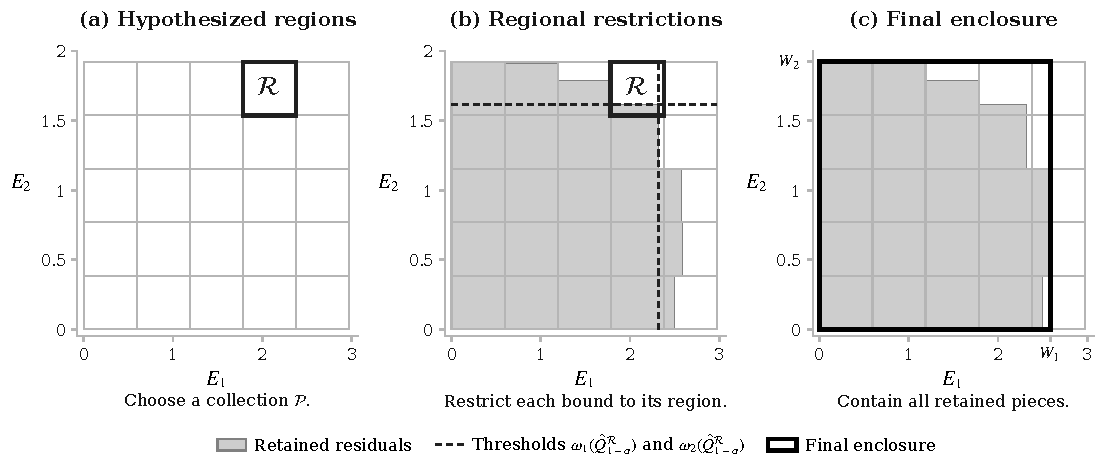
\includegraphics[width=\linewidth]{blueprint_regional_construction.pdf}
    \caption{An illustration of a regional-union construction in the residual space using absolute residuals with $n=10$ and $\alpha=0.1$.
    (a) A collection $\mathcal P$ of hypothesized residual regions, with one region $\mathcal R$ highlighted.
    (b) Each shaded piece is the intersection of its region with the constraints $0\leq z_j\leq\omega_j(\hat Q^{\mathcal R}_{1-\alpha})$ for $j=1,2$; the dashed lines show the thresholds for the highlighted region.
    (c) A coordinatewise enclosure of this union contains every retained piece. This figure only illustrates the idea of the regional-union argument; the practical construction described below uses a different $\mathcal{P}$.}
    \label{fig:regional-construction-blueprint}
\end{figure}

The main technical challenges from these three steps are (1) how to define suitable link functions, (2) how to find a suitable collection of subregions $\mathcal{P}$, (3) how $\hat Q^{\mathcal{R}}_{1-\alpha}$ is defined, and (4) how to obtain a final prediction set with a simple and interpretable coordinatewise structure with marginal coverage.
We will address these challenges in the following subsections, and then summarize the final practical construction at the end.

\subsection{Explicit Form of the Link Functions}\label{sec:link-functions}

In this section, we present the explicit form of the link functions $\omega_1,\ldots,\omega_d$ defined implicitly in~\eqref{eq:key-ineq}, along with their guarantee.
For the constructions below, take $n\geq2$. Define the observed statistics $\hat{\boldsymbol\mu}^{\mathrm{obs}}$ and $\hat{\boldsymbol\sigma}^{\mathrm{obs}}$ as

\begin{equation} \label{eq:plug-in-mean-std}
\begin{aligned}
\hat{\boldsymbol\mu}^{\mathrm{obs}}
&=(\hat\mu^{\mathrm{obs}}_1,\ldots,\hat\mu^{\mathrm{obs}}_d)^\top,
\quad
\hat{\boldsymbol\sigma}^{\mathrm{obs}}
=(\hat\sigma^{\mathrm{obs}}_1,\ldots,\hat\sigma^{\mathrm{obs}}_d)^\top,\\
\hat\mu^{\mathrm{obs}}_j
&=\frac1n\sum_{i=1}^n E^i_j,
\quad
\hat\sigma^{\mathrm{obs}}_j
=\sqrt{\frac1n\sum_{i=1}^n\!\bigl(E^i_j-\hat\mu^{\mathrm{obs}}_j\bigr)^2}.
\end{aligned}
\end{equation}
Note that we use the factor $1/n$ instead of $1/(n-1)$ in the definition of $\hat{\boldsymbol\sigma}^{\mathrm{obs}}$ for algebraic simplicity.
Assumption~\ref{eq:assumption-scores} ensures $\hat\sigma^{\mathrm{obs}}_j>0$ almost surely for all $j\in[d]$.

The explicit form of $\omega_j(c)$ is given in the following lemma.

\begin{lemma}\label{lem:solution-key-ineq}
Under Assumption~\ref{eq:assumption-scores}, suitable link functions $\omega_1,\ldots,\omega_d$ satisfying~\eqref{eq:key-ineq} are
\[
\omega_j(c)
=\begin{cases}
-\infty,&\text{if }c\leq-T,\\[3pt]
\displaystyle
\hat\mu^{\mathrm{obs}}_j+c\hat\sigma^{\mathrm{obs}}_j
\sqrt{\dfrac{n+1}{T^2-c^2}},
&\text{if }-T<c<T,\\[6pt]
+\infty,&\text{if }c\geq T,
\end{cases}
\qquad T=\frac{n}{\sqrt{n+1}}.
\]
The first and last cases also define $\omega_j(-\infty)=-\infty$ and $\omega_j(+\infty)=+\infty$.
\end{lemma}

Substituting this expression for the link functions into~\eqref{eq:hat-set-valued-map} and setting $c=\hat Q^{\mathrm{oracle}}_{1-\alpha}$ gives an oracle upper bound $\omega_j(\hat Q^{\mathrm{oracle}}_{1-\alpha})$ for $E_j(\mathbf X^{n+1},y_j)$. These upper bounds are real-valued when $-T<\hat Q^{\mathrm{oracle}}_{1-\alpha}<T$. The following lemma gives a sufficient sample-size condition on this.

\begin{lemma}
Under Assumption~\ref{eq:assumption-scores}, if $n\geq\max\{3,1/\alpha-1\}$, then $|\hat Q^{\mathrm{oracle}}_{1-\alpha}|<n/\sqrt{n+1}$ almost surely.
\label{lem:finite-prediction-guarantee}
\end{lemma}

Thus, the oracle residual thresholds $\omega_j(\hat Q^{\mathrm{oracle}}_{1-\alpha})$ are finite almost surely under the stated sample-size condition, which is mild and commonly satisfied in practice. The same sample size condition also ensures finiteness of the practical thresholds introduced in the next section, so we will revisit this lemma again but in a slightly different format. 

\subsection{Approximation of the Transductive Oracle with Pseudo Upper Bounds}\label{sec:practical-approximation}

We obtain the \emph{pseudo upper bound} $\hat Q^{\mathcal R}_{1-\alpha}$ by assuming $\mathbf E^{n+1}\in\mathcal R$ for some subregion $\mathcal R\subseteq\R^d$ and taking worst-case upper bounds of the standardized residuals used to compute $\hat Q^{\mathrm{oracle}}_{1-\alpha}$ over all possible values of $\mathbf E^{n+1}\in\mathcal R$.

To simplify the derivation, we also require $\mathcal R$ to be a nonempty hyper-rectangle, that is, $\mathcal R=\bigtimes_{j=1}^d I_j$, where each $I_j\subseteq\R$ is a nonempty interval with endpoints $l_j:=\inf I_j$ and $u_j:=\sup I_j$. Finite endpoints may be included or excluded, and unbounded intervals are allowed. By continuity, the inclusion or exclusion of a finite endpoint does not change the supremum below.

Let $\mathbf z$ denote a placeholder for the test residual $\mathbf E^{n+1}$.
Define the pseudo location and scale parameters
$\hat{\boldsymbol\mu}(\mathbf z):=(\hat\mu_1(z_1),\ldots,\hat\mu_d(z_d))^\top$
and
$\hat{\boldsymbol\sigma}(\mathbf z):=(\hat\sigma_1(z_1),\ldots,\hat\sigma_d(z_d))^\top$
as if $\mathbf E^{n+1}$ in~\eqref{eq:transductive-oracle-mean-std} were replaced by $\mathbf z$:
\begin{align}\label{eq:placeholder-mean-std}
\hat\mu_j(z_j)
&=
\frac{\sum_{i=1}^nE_j^i+z_j}{n+1},
\qquad
\hat\sigma_j(z_j)
=
\sqrt{
\frac{
\bigl(z_j-\hat\mu_j(z_j)\bigr)^2
+
\sum_{i=1}^n\!\bigl(E_j^i-\hat\mu_j(z_j)\bigr)^2
}{n}
}.
\end{align}
By plugging in $\mathbf z=\mathbf E^{n+1}$, we have
$\hat{\boldsymbol\mu}(\mathbf E^{n+1})=\hat{\boldsymbol\mu}^{\mathrm{oracle}}$
and
$\hat{\boldsymbol\sigma}(\mathbf E^{n+1})=\hat{\boldsymbol\sigma}^{\mathrm{oracle}}$.

Suppose now that $\mathbf E^{n+1}\in\mathcal R$ for some hyper-rectangle $\mathcal R\subseteq\R^d$, which we refer to as our working hypothesis. We can then define a pseudo transformation $\Phi^{\mathcal R}:\R^d\to\R$, tailored to this hypothesis, by considering the most unfavorable (largest) possible value of the standardized ratio as a function of $E_j^{n+1}=z_j\in I_j$:
\begin{equation}\label{eq:pseudo-transformation}
\Phi^{\mathcal R}(\mathbf t)
:=
\max_{1\leq j\leq d}
\sup_{z_j\in I_j}
\frac{t_j-\hat\mu_j(z_j)}{\hat\sigma_j(z_j)},
\qquad
\mathbf t\in\R^d.
\end{equation}
This definition does not require the working hypothesis. Under the working hypothesis, however, the supremum includes $z_j=E_j^{n+1}$ for every $j\in[d]$, so $\Phi^{\mathcal R}$ is guaranteed to be at least as large as the oracle transformation:
\[
\Phi^{\mathcal R}(\mathbf t)
\geq
\Phi^{\mathrm{oracle}}(\mathbf t),
\qquad
\forall\mathbf t\in\R^d.
\]

Conveniently, $\Phi^{\mathcal R}$ admits a closed-form expression.
\begin{lemma}\label{lem:pseudo-transformation}
Under Assumption~\ref{eq:assumption-scores}, for each $j\in[d]$, define
\[
M_j^{\mathcal R}(t_j)
:=
\begin{cases}
\displaystyle
\sqrt{
\frac{(t_j-\hat\mu_j^{\mathrm{obs}})^2}
{(\hat\sigma_j^{\mathrm{obs}})^2}
+\frac1{n+1}
},
&
\begin{array}{l}
\text{if }t_j>\hat\mu_j^{\mathrm{obs}}\text{ and}
\\
l_j\leq
\hat\mu_j^{\mathrm{obs}}
-
\frac{(\hat\sigma_j^{\mathrm{obs}})^2}
{t_j-\hat\mu_j^{\mathrm{obs}}}
\leq u_j,
\end{array}
\\[12pt]
-\infty,
&\text{otherwise}.
\end{cases}
\]
The pseudo transformation $\Phi^{\mathcal R}$ defined in~\eqref{eq:pseudo-transformation} can be written as
\[
\Phi^{\mathcal R}(\mathbf t)
=
\max_{1\leq j\leq d}
\max\left\{
\frac{t_j-\hat\mu_j(l_j)}{\hat\sigma_j(l_j)},
\quad
M_j^{\mathcal R}(t_j),
\quad
\frac{t_j-\hat\mu_j(u_j)}{\hat\sigma_j(u_j)}
\right\}.
\]
In addition, if $l_j=-\infty$ or $u_j=+\infty$ for any $j\in[d]$, the corresponding endpoint term is interpreted using
\[
\lim_{z_j\to-\infty}
\frac{t_j-\hat\mu_j(z_j)}{\hat\sigma_j(z_j)}
=
\frac1{\sqrt{n+1}},
\qquad
\lim_{z_j\to+\infty}
\frac{t_j-\hat\mu_j(z_j)}{\hat\sigma_j(z_j)}
=
-\frac1{\sqrt{n+1}}.
\]
\end{lemma}

Using Lemma~\ref{lem:pseudo-transformation}, we can define the pseudo upper bound
$\hat Q^{\mathcal R}_{1-\alpha}:=\hat Q_{1-\alpha}(S^1_{\mathcal R},\ldots,S^n_{\mathcal R})$,
where $S^i_{\mathcal R}=\Phi^{\mathcal R}(\mathbf E^i)$ for all $i\in[n]$. Then, under the working hypothesis $\mathbf E^{n+1}\in\mathcal R$, we have $\hat Q^{\mathcal R}_{1-\alpha}\geq\hat Q^{\mathrm{oracle}}_{1-\alpha}$ because $\Phi^{\mathcal R}\geq\Phi^{\mathrm{oracle}}$ uniformly.
Substituting $c=\hat Q^{\mathcal R}_{1-\alpha}$ into~\eqref{eq:hat-set-valued-map} and intersecting the resulting prediction set with $\{\mathbf y:\mathbf E(\mathbf X^{n+1},\mathbf y)\in\mathcal R\}$, we obtain the regional prediction set $\hat C^{\mathcal R}(\mathbf X^{n+1})$ defined in~\eqref{eq:pseudo-prediction-set}.
Algorithm~\ref{alg:pseudo-prediction-set} summarizes the procedure in detail. 

\begin{algorithm}[!htbp]
\caption{Construction of regional prediction sets under the working hypothesis $\mathbf E^{n+1}\in\mathcal R$}
\label{alg:pseudo-prediction-set}

\textbf{Input:} Calibration residuals $\{\mathbf E^i\}_{i=1}^n$; test input $\mathbf X^{n+1}$; target miscoverage level $\alpha\in(0,1)$; nonempty hyper-rectangle $\mathcal R=\bigtimes_{j=1}^d I_j$.

\begin{algorithmic}[1]
\State Compute $\hat{\boldsymbol\mu}^{\mathrm{obs}}$ and $\hat{\boldsymbol\sigma}^{\mathrm{obs}}$ using~\eqref{eq:plug-in-mean-std}.
\State Compute $S^i_{\mathcal R}=\Phi^{\mathcal R}(\mathbf E^i)$ \textbf{for} $i\in[n]$ using $\Phi^{\mathcal R}$ defined in Lemma~\ref{lem:pseudo-transformation}.
\State Compute $\hat Q^{\mathcal R}_{1-\alpha}:=\hat Q_{1-\alpha}(S^1_{\mathcal R},\ldots,S^n_{\mathcal R})$.
\State Compute $\omega_1(\hat Q^{\mathcal R}_{1-\alpha}),\ldots,\omega_d(\hat Q^{\mathcal R}_{1-\alpha})$ using $\omega_1,\ldots,\omega_d$ defined in Lemma~\ref{lem:solution-key-ineq}.
\State Construct
\[
\hat C(\mathbf X^{n+1};\hat Q^{\mathcal R}_{1-\alpha})
=
\left\{
\mathbf y:
a_j(\mathbf X^{n+1})
\leq E_j(\mathbf X^{n+1},y_j)
\leq\omega_j(\hat Q^{\mathcal R}_{1-\alpha})
\text{ for all }j\in[d]
\right\}.
\]
\State \Return
\[
\hat C^{\mathcal R}(\mathbf X^{n+1})
:=
\hat C(\mathbf X^{n+1};\hat Q^{\mathcal R}_{1-\alpha})
\cap
\left\{
\mathbf y:
\mathbf E(\mathbf X^{n+1},\mathbf y)\in\mathcal R
\right\}.
\]
\end{algorithmic}
\end{algorithm}

The following lemma establishes the guarantee of the regional prediction set $\hat C^{\mathcal R}(\mathbf X^{n+1})$ under the working hypothesis $\mathbf E^{n+1}\in\mathcal R$, as promised in Section~\ref{sec:blueprint}:

\begin{lemma}\label{lem:pseudo-guarantee}
Under Assumption~\ref{eq:assumption-scores}, the regional prediction set $\hat C^{\mathcal R}(\mathbf X^{n+1})$ constructed by Algorithm~\ref{alg:pseudo-prediction-set} satisfies
~\eqref{eq:pseudo-implication}.
\end{lemma}

\begin{proof}
If $\mathbf Y^{n+1}\in\hat C(\mathbf X^{n+1};\hat Q^{\mathrm{oracle}}_{1-\alpha})$, then $E_j^{n+1}\leq\omega_j(\hat Q^{\mathrm{oracle}}_{1-\alpha})$ for all $j\in[d]$. Under the additional hypothesis that $\mathbf E^{n+1}\in\mathcal R$, we know that $\hat Q^{\mathcal R}_{1-\alpha}\geq\hat Q^{\mathrm{oracle}}_{1-\alpha}$. Hence, $\omega_j(\hat Q^{\mathrm{oracle}}_{1-\alpha})
\leq
\omega_j(\hat Q^{\mathcal R}_{1-\alpha})$
for all $j\in[d]$ because $\omega_1,\ldots,\omega_d$ are nondecreasing functions. Therefore, we have $E_j^{n+1}\leq\omega_j(\hat Q^{\mathcal R}_{1-\alpha})$ for all $j\in[d]$, which is exactly the condition
$\mathbf Y^{n+1}\in\hat C(\mathbf X^{n+1};\hat Q^{\mathcal R}_{1-\alpha})$,
under the hypothesis that $\mathbf E^{n+1}\in\mathcal R$. Intersecting these two events yields $\mathbf Y^{n+1}\in\hat C^{\mathcal R}(\mathbf X^{n+1})$.
\end{proof}

In general, guaranteeing~\eqref{eq:pseudo-implication} does not imply marginal coverage for $\hat C^{\mathcal R}(\mathbf X^{n+1})$, because the working hypothesis $\mathbf E^{n+1}\in\mathcal R$ may occur with very low probability. 
As we previewed in Section~\ref{sec:blueprint}, we will resolve this by finding a collection of subregions $\mathcal R$ whose union contains $\mathbf E^{n+1}$ whenever the oracle coverage event occurs, described in~\eqref{eq:subregions-requirement}. If such a collection can be found, Lemma~\ref{lem:pseudo-guarantee} then further implies that the union of their corresponding regional prediction sets preserves the same oracle coverage event.

The shortcoming of doing so naively is that such a union might not be a rectangle even for standard choices of residuals, which would violate our promise of interpretability (revisit Figure~\ref{fig:regional-construction-blueprint} for an example). We will use a full-cell regional union as a benchmark and construct practical coordinatewise upper bounds that enclose it. The coverage proof for the practical bounds will follow directly from preservation of the same oracle coverage event.

Before constructing these regions, we give the separate guarantee needed for finite practical residual thresholds, as promised earlier.

\begin{lemma}\label{lem:regional-finite-bounds}
Under Assumption~\ref{eq:assumption-scores}, if
$n\geq\max\{3,1/\alpha-1\}$, then $|\hat Q^{\mathcal R}_{1-\alpha}|<n/\sqrt{n+1}$ almost surely
for every nonempty rectangular region $\mathcal R$, including random regions. Consequently, all corresponding link values
$\omega_j(\hat Q^{\mathcal R}_{1-\alpha})$ are finite almost surely.
\end{lemma}

\subsection{A Data-Dependent Collection and Hyper-Rectangular Enclosure}\label{sec:collection}

The goal in this section is to find a collection of subregions $\mathcal P$ that satisfies~\eqref{eq:subregions-requirement} and to outline the structure of the final prediction set. We first construct a coarse prediction set using a single region containing all possible test residuals. Its retained residuals then provide a potentially smaller region within which we can refine the construction of subregions while preserving the oracle coverage event.

For simplicity of derivation, we denote the retained residuals corresponding to $\hat C^{\mathcal R}(\mathbf X^{n+1})$ by
\begin{equation}\label{eq:retained-residuals}
Z^{\mathcal R}
:=
\left\{
\mathbf z\in\R^d:
a_j(\mathbf X^{n+1})
\leq z_j\leq\omega_j(\hat Q^{\mathcal R}_{1-\alpha})
\text{ for all }j\in[d]
\right\}
\cap\mathcal R,
\end{equation}
which satisfies
$\mathbf y\in\hat C^{\mathcal R}(\mathbf X^{n+1})$
if and only if
$\mathbf E(\mathbf X^{n+1},\mathbf y)\in Z^{\mathcal R}$.

Before we discuss the construction of the collection of subregions, we introduce the following definition.

\begin{definition}[Finite Inner Cover]
A finite inner cover of a set $A$ is a collection of sets
$\{P_1,P_2,\ldots,P_k\}$ such that $P_i\subseteq A$ for all $i\in[k]$ and
$A=\bigcup_{i=1}^k P_i$.
We allow the empty collection as a finite inner cover of the empty set.
\end{definition}

Therefore, to guarantee~\eqref{eq:subregions-requirement}, we can take $\mathcal P$ to be a finite inner cover of $D$, with the restriction that all of its elements are hyper-rectangles. However, $D$ is still an unbounded region to consider initially, so we want to find a smaller subset of $D$ such that~\eqref{eq:subregions-requirement} is preserved if we choose $\mathcal P$ to be a finite inner cover of that smaller subset. Fortunately, our regional prediction set provides this refinement.

\paragraph{One-step Refinement} Let $D$ be the smallest \emph{fixed} domain of residuals out of our knowledge. For example, we would choose $D=\R^d_+$ for absolute residuals and $D=\R^d$ for quantile residuals. Our method would still work if $D = \R^d$ is selected for absolute residual case, at a cost of unnecessary potential conservatism. The purpose of having a fixed domain $D$ is to avoid recomputation for every new test input.

Applying the regional construction in Algorithm~\ref{alg:pseudo-prediction-set} with $\mathcal R=D$ gives the prediction set $\hat C^D(\mathbf X^{n+1})$, whose retained residuals are, by~\eqref{eq:retained-residuals},
\[
Z^D
=
\bigtimes_{j=1}^d Z_j^D,
\qquad
Z_j^D:=
\left[
a_j(\mathbf X^{n+1}),
\omega_j(\hat Q^D_{1-\alpha})
\right]\cap\R.
\]
This is a hyperrectangle, possibly empty. Under the sample-size condition in Lemma~\ref{lem:regional-finite-bounds}, it is bounded above almost surely. Since the test residual belongs to $D$ almost surely, Lemma~\ref{lem:pseudo-guarantee} gives
\[
\mathbf Y^{n+1}\in
\hat C(\mathbf X^{n+1};\hat Q^{\mathrm{oracle}}_{1-\alpha})
\implies
\mathbf E^{n+1}\in Z^D\subseteq D.
\]
Hence, by choosing $\mathcal P$ to be a finite inner cover of $Z^D$, we preserve~\eqref{eq:subregions-requirement}. If $Z^D=\varnothing$, we set $\mathcal P=\varnothing$ and $W_j=-\infty$ for every $j$, and return the empty prediction set. No further regional thresholds need to be computed. In the remainder of the construction, suppose that $Z^D\neq\varnothing$.

{\color{brown}
The choice of a fixed initial domain $D$ also has a computational benefit. By substituting $\mathcal R$ with $D$, rather than the input-dependent lower-bound region, the coordinatewise upper residual thresholds $\omega_j(\hat Q^D_{1-\alpha})$ remain fixed for all test inputs. Having this structure allows us to compute these quantities once from the observed residuals and reuse them across test inputs, which is crucial for practical implementation. The lower bounds $a_j(\mathbf X^{n+1})$ may still depend on the test input, but they are easy to compute for absolute and quantile residuals. Consequently, $Z^D$ and the subsequent regional calculations may change even though the global upper thresholds are reused.
}

We will construct the finite inner covers using the observed calibration residuals, with the aim of obtaining tighter regional bounds while keeping the number of additional regional calculations manageable.

For each $j\in[d]$, let $N_j$ denote the number of calibration residual values $E_j^1,\ldots,E_j^n$ strictly inside $Z_j^D$, and let
$\eta_j^1<\cdots<\eta_j^{N_j}$
denote these values in increasing order (they are distinct under Assumption~\ref{eq:assumption-scores}). Thus, $0\leq N_j\leq n$ and
$a_j(\mathbf X^{n+1})=:
\eta_j^0\leq \eta_j^1<\cdots<
\eta_j^{N_j}\leq \eta_j^{N_j+1}:=\omega_j(\hat Q^D_{1-\alpha}).$
Define
\begin{equation}\label{eq:interval-partition}
    I_j^h:=[\eta_j^{h-1},\eta_j^h)\cap\R, h \in [N_j],\qquad I_j^{N_j+1}:=
    [\eta_j^{N_j},\eta_j^{N_j+1}] \cap \R,
\end{equation}
then
$\{I_j^h\}^{N_j+1}_{h=1}$
forms a partition of $Z_j^D$ into $N_j+1$ disjoint intervals. In particular, when $N_j=0$, this partition consists of the single interval $I_j^1=Z_j^D$.

These breakpoints use the observed residual values to provide a data-dependent partition in each coordinate, with at most $n+1$ intervals. Below, we first provide a direct construction of the finite inner cover whose explicit evaluation can be computationally expensive.

\paragraph{The Full-Cell Benchmark}

Because each $\{I_j^h\}^{N_j+1}_{h=1}$ partitions $Z_j^D$, taking all products of the coordinate intervals gives a finite inner cover of $Z^D$:
\begin{equation}\label{eq:full-cell-partition}
\mathcal P_{\mathrm{full}}
:=
\left\{
\bigtimes_{j=1}^d I_j^{h_j}:
h_j\in[N_j+1]\text{ for all }j\in[d]
\right\}.
\end{equation}
For each cell $\mathcal{R} \in \mathcal P_{\mathrm{full}}$, we can apply the regional construction in Algorithm~\ref{alg:pseudo-prediction-set} and retain its corresponding residuals $Z^\mathcal{R}$ defined in~\eqref{eq:retained-residuals}. Taking their union and its coordinatewise upper bounds gives
\begin{equation}\label{eq:full-cell-benchmark}
\mathcal U_{\mathrm{full}}
:=
\bigcup_{\mathcal R\in\mathcal P_{\mathrm{full}}}Z^{\mathcal R}
\subseteq Z^D,
\qquad
W_j^{\mathrm{full}}
:=
\sup_{\mathbf z\in\mathcal U_{\mathrm{full}}}z_j,
\quad j\in[d],
\end{equation}
with $\sup\varnothing:=-\infty$. Since $\mathcal P_{\mathrm{full}}$ is a finite inner cover of $Z^D$, Lemma~\ref{lem:pseudo-guarantee} ensures that this union contains the test residual whenever the oracle coverage event occurs. Therefore, $\bigtimes_{j=1}^d
\left(
[a_j(\mathbf X^{n+1}),W_j^{\mathrm{full}}]\cap\R
\right)$
gives a hyper-rectangular enclosure that preserves the same event. It is also the smallest closed hyper-rectangle of this form enclosing this union.

However, explicitly evaluating every cell requires considering $|\mathcal P_{\mathrm{full}}|=\prod_{j=1}^d(N_j+1)\leq(n+1)^d$ regions, which can be computationally infeasible even for moderate $d$. We therefore use this construction as a benchmark and seek an enclosure without explicitly evaluating every cell. Our practical construction restricts only one coordinate at a time, while allowing the other coordinates to range over $Z^D$. In general, doing so would result in looser upper bounds on the residuals because we shift from restricting all coordinates together in each cell to just one of them at a time, but we will show empirically that under our particular construction, the difference is minimal. Moreover,
Proposition~\ref{prop:envelope-tightness} will give a sufficient condition under which the thresholds from our construction will agree exactly with those of the full-cell benchmark.

\subsection{Efficient Approximation of the Thresholds}

For each coordinate $j\in[d]$, we construct a \emph{coordinatewise cover} of $Z^D$ by partitioning that coordinate only. Specifically, for $h\in[N_j+1]$, define
\begin{equation}\label{eq:coordinate-envelope-region}
\mathcal R_j^h
:=
Z_1^D\times\cdots\times Z_{j-1}^D
\times I_j^h
\times Z_{j+1}^D\times\cdots\times Z_d^D.
\end{equation}
The collection $\mathcal P_j(Z^D):=\{\mathcal R_j^h:h\in[N_j+1]\}$ clearly satisfies $\bigcup_{h=1}^{N_j+1}\mathcal R_j^h=Z^D$ and hence forms a finite inner cover of $Z^D$. Together, we have constructed $d$ finite inner covers, using at most $\sum_{j=1}^d(N_j+1)\leq d(n+1)$ regions.

We use the cover $\mathcal P_j(Z^D)$ to obtain an upper bound for coordinate $j$ only. For this purpose, define the union of its retained residual sets and the corresponding upper bound by
\begin{equation}\label{eq:envelope-upper-endpoints}
\mathcal U_j
:=
\bigsqcup_{h=1}^{N_j+1}Z^{\mathcal R_j^h},
\qquad
W_j
:=
\sup_{\mathbf z\in\mathcal U_j}z_j,
\quad j\in[d],
\end{equation}
again with $\sup\varnothing:=-\infty$. See Figure~\ref{fig:data-dependent-collection} for illustration.

\begin{figure}[!htbp]
    \centering
    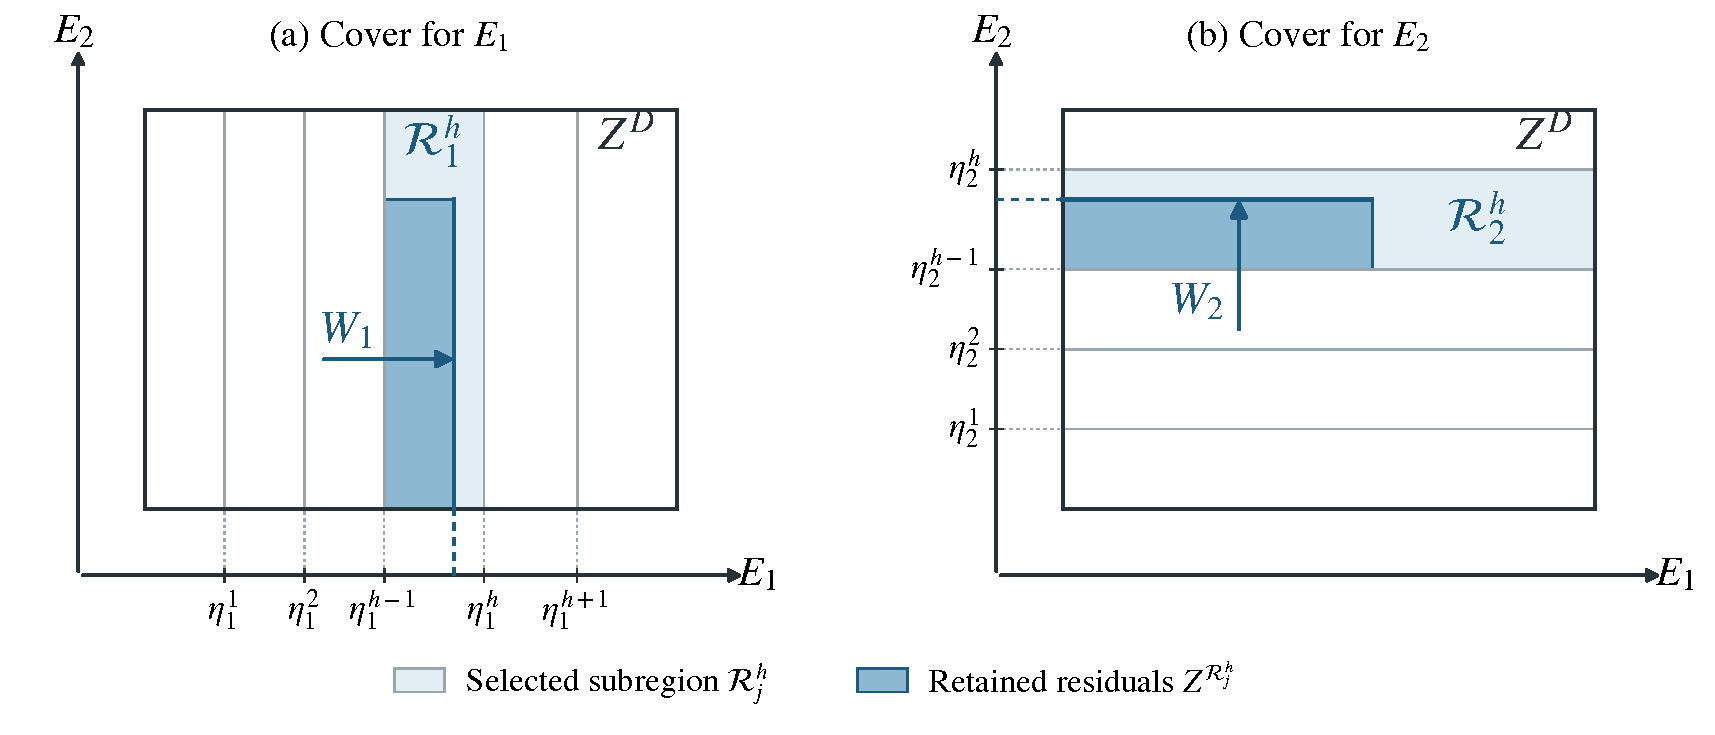
\includegraphics[width=\linewidth]{data_dependent_collection.pdf}
    \caption{The data-dependent coordinatewise covers of $Z^D$ in two dimensions. The calibration residuals inside each coordinate interval $Z_j^D$ determine the interior breakpoints $\eta_j^h$, producing vertical slabs for the first coordinate (left) and horizontal slabs for the second coordinate (right). The arrows mark the resulting coordinatewise upper bounds $W_1$ and $W_2$.}
    \label{fig:data-dependent-collection}
\end{figure}


For every $j\in [d]$, the cover $\mathcal P_j(Z^D)$ satisfies~\eqref{eq:subregions-requirement}, so the test residual belongs to $\mathcal U_j$ for every $j$ whenever the oracle coverage event occurs. This further implies
\begin{equation}\label{eq:practical-implication}
    \mathbf Y^{n+1} \in \hat{C}(\mathbf X^{n+1}; \hat{Q}^\mathrm{oracle}_{1-\alpha}) \implies \mathbf E^{n+1} \in \bigcap^d_{j=1}\mathcal U_j \implies \mathbf E^{n+1} \in \bigtimes^d_{j=1}[a_j(\mathbf X^{n+1}), W_j].
\end{equation}

The last piece in~\eqref{eq:practical-implication} where the test residual belongs is clearly a hyper-rectangle in the residual space, so we can complete our prediction set construction by finding $(W_1,\ldots, W_d)$. The following lemma provides an explicit algorithm for this task.

\begin{lemma}\label{lem:upper-endpoints}
    Assume Assumption~\ref{eq:assumption-scores} holds. For every $j\in [d]$, let $h^* \in [N_j+1]$ be the largest index such that $Z^{\mathcal R_j^{h^*}} \neq \emptyset$, then $W_j$ defined in~\eqref{eq:envelope-upper-endpoints} can be described explicitly by
    \[
    W_j = \sup_{\mathbf z\in Z^{\mathcal R_j^{h^*}}}z_j=\min\left\{\eta_j^{h^*},\omega_j\left( \hat Q^{\mathcal R_j^{h^*}}_{1-\alpha}\right)\right\}.
    \]
    If no such $h^*$ exists, $W_j = -\infty$. Moreover, $W_j = W^\mathrm{full}_j$ for all $j\in [d]$.
\end{lemma}

Using Lemma~\ref{lem:upper-endpoints}, we can construct the prediction set of our \emph{transductively standardized conformal prediction} (TSCP) method as
\begin{equation}\label{eq:TSCP}
\hat C^{\mathrm{TSCP}}(\mathbf X^{n+1})
:=
\left\{\mathbf y\in\R^d:
a_j(\mathbf X^{n+1})
\leq E_j(\mathbf X^{n+1},y_j)\leq W_j
\text{ for all }j\in[d]\right\}.
\end{equation}
Algorithm~\ref{alg:coordinatewise-bounds} summarizes this entire procedure. This algorithm can be implemented at a cost of $\mathcal{O}(dn^2)$. See Appendix~\ref{app:lwc-sc-cost} for details.

\begin{algorithm}[!htbp]
\caption{Transductively Standardized Conformal Prediction (TSCP)}
\label{alg:coordinatewise-bounds}
\textbf{Input:} Calibration residuals $\{\mathbf E^i\}_{i=1}^n$; test input $\mathbf X^{n+1}$; target miscoverage level $\alpha\in(0,1)$; Algorithm~\ref{alg:pseudo-prediction-set}; fixed residual domain $D$.
\begin{algorithmic}[1]
\State Compute $\Phi^D(t) = \max_{1\leq j\leq d}\Phi^D_j(t)$ by Lemma~\ref{lem:pseudo-transformation}.
\State Construct $\hat C^D(\mathbf X^{n+1})$ using Algorithm~\ref{alg:pseudo-prediction-set} and $Z^D = \bigtimes^d_{j=1}Z^D_j$ using~\eqref{eq:retained-residuals}.
\If{$Z^D=\varnothing$}
    \State \Return $\hat C^{\mathrm{TSCP}}(\mathbf X^{n+1}):=\varnothing$.
\EndIf
\For{$j=1,\ldots,d$}
    \State $W_j\gets-\infty$.
    \State Compute $N_j = \sum^n_{i=1}\mathbb{I}\{a_j(\mathbf X^{n+1})<E^i_j<\omega_j(\hat Q^D_{1-\alpha})\}$. 
    \State Construct $I_j^1,\ldots,I_j^{N_j+1}$ using~\eqref{eq:interval-partition}.
    \For{$h=N_j+1,N_j,\ldots,1$}
        \State Construct $\mathcal{R}^h_j$ using~\eqref{eq:coordinate-envelope-region}.
        \State Construct $\hat C^{\mathcal{R}^h_j}(\mathbf X^{n+1})$ using Algorithm~\ref{alg:pseudo-prediction-set} and $Z^{\mathcal{R}^h_j}$ using~\eqref{eq:retained-residuals}.
        \If{$Z^{\mathcal R_j^h}\neq\varnothing$}
            \State
            $\displaystyle
            W_j\gets
            \min\left\{\eta_j^h,
            \omega_j(\hat Q^{\mathcal R_j^h}_{1-\alpha})\right\}$.
            \State \textbf{break}.
        \EndIf
    \EndFor
\EndFor
\State \Return 
\[
\hat C^{\mathrm{TSCP}}(\mathbf X^{n+1})
:=
\left\{\mathbf y\in\R^d:
a_j(\mathbf X^{n+1})
\leq E_j(\mathbf X^{n+1},y_j)\leq W_j
\text{ for all }j\in[d]\right\}.
\]
\end{algorithmic}
\end{algorithm}


Proposition~\ref{prop:TSCP} establishes the fact that $\mathbf Y^{n+1} \in \hat C^{\mathrm{TSCP}}(\mathbf X^{n+1})$ whenever the oracle coverage event occurs, hence inheriting its marginal coverage from Theorem~\ref{thm:fixed-transformation-coverage}.



\begin{proposition}\label{prop:TSCP}
Under Assumption~\ref{eq:assumption-scores}, the TSCP prediction set $\hat C^{\mathrm{TSCP}}(\mathbf X^{n+1})$ defined in~\eqref{eq:TSCP} satisfies
\[
\mathbf Y^{n+1}\in
\hat C(\mathbf X^{n+1};\hat Q^{\mathrm{oracle}}_{1-\alpha})
\implies
\mathbf Y^{n+1}\in
\hat C^{\mathrm{TSCP}}(\mathbf X^{n+1}).
\]
\end{proposition}

\subsection{Tightness of TSCP}\label{sec:tightness}




\clearpage
% Main numerical experiments.
% Required packages: amsmath, booktabs, graphicx, and xcolor.
% Figure paths are relative to this file's directory.

\begingroup
\color{blue}
\setlength{\emergencystretch}{2em}

\FloatBarrier
\section{Numerical Experiments}
\label{sec:numerical-experiments}
\label{sec:experiments}

We evaluate Transductively Standardized Conformal Prediction (TSCP) on
simulated and real multivariate regression problems, studying joint coverage,
coordinate-wise interval length, prediction-set volume, and computational cost. 
We first consider absolute-residual scores under independent Gaussian noise
to establish the effect of unequal outcome scales, followed by dependent
and partially heteroskedastic noise to examine cross-output and
input-dependent variation. We then study quantile-regression scores and
six real datasets. Appendix~\ref{app:additional-experiments} provides
additional noise-distribution comparisons, sensitivity analyses, heavy-tail
and contamination stress tests, and comparisons with the oracle and
alternative constructions introduced in the paper.

\subsection{Methods and Evaluation Metrics}
\label{sec:experiment-methods}

The primary comparisons use four methods. \emph{Unscaled Max} applies split
conformal prediction to the maximum coordinate-wise residual without
additional scaling. \emph{Point CHR} estimates coordinate scales using an
additional data split \citep{sampson2024conformal}. \emph{Emp.
Copula} estimates a dependence model from the calibration residuals and then
uses the same observations for calibration; this implementation does not have
the finite-sample guarantee enjoyed by the other methods
\citep{messoudi2021copula}. \emph{TSCP} denotes
the rectangular local-worst-case construction proposed in Algorithm~\ref{alg:shortcut}. For
quantile-regression experiments, we replace Point CHR with the native
quantile-hyperrectangle method \emph{CQHR} of
\citet{sampson2024conformal}. Appendix~\ref{app:shape-template} contains a
separate low-dimensional comparison with the hyperrectangular shape-template
method of \citet{tumu2024templates}.

For a test sample of size $m$, we report the empirical joint coverage
\[
  \widehat{\operatorname{Cov}}
  = \frac{1}{m}\sum_{i=1}^{m}
    \mathbf{1}\!\left\{\boldsymbol{Y}_i
    \in \widehat{C}(\boldsymbol{X}_i)\right\}.
\]
For absolute-residual experiments, all methods return a rectangle with residual
half-widths $(\mathcal{L}_1,\ldots,\mathcal{L}_d)$. We therefore report the normalized
residual-space volume $\prod_{j=1}^{d}\mathcal{L}_j$, which equals $2^{-d}$ times the
full rectangular volume in the outcome space, and the full coordinate-wise interval lengths
$2\mathcal{L}_j$. For quantile-regression experiments, the base interval
depends on the test covariates, so volume and coordinate lengths are
averaged over the test observations in outcome space. Runtime is
the wall-clock time needed to construct the conformal region after residuals
have been computed; fitting the underlying regression model is excluded. Unless
stated otherwise, absolute-residual results are averaged over 200 repetitions (30 repetitions for quantile-regression experiments)
and the target coverage is $1-\alpha=0.9$. All methods in each repetition use
the same fitted regression model, calibration observations, and test observations.
Sample sizes and model settings are specified below. 

\subsection{Absolute Mean-Regression Residuals}
\label{sec:absolute-residual-experiments}

We first generate $10$-dimensional features
$\boldsymbol{X}\sim\mathcal{N}(\boldsymbol{0},I_{10})$ and outcomes
\begin{equation}
  Y_j=f_j(\boldsymbol X)+\epsilon_j,\qquad j\in[d],
  \label{eq:data-generator}
\end{equation}
where $d=10$ and every $f_j$ is linear, with coefficients sampled once
from $\operatorname{Unif}(-10,10)$ and held fixed across repetitions.
In each repetition, we independently generate 7,200 training observations,
800 test observations, and a calibration sample of size $n\in\{30,50,100,300,500\}$. We
estimate the regression coefficients using
ordinary least squares, and all methods in each repetition share the same fitted predictor. 

\subsubsection{Independent Gaussian Noise}

Figure~\ref{fig:gaussian-heter} reports results under independent Gaussian
noise with $\epsilon_j\sim\mathcal{N}(0,(11-j)^2)$ for $j\in[10]$. TSCP
combines near-nominal joint coverage with smaller prediction-set volumes
than Point CHR and Unscaled Max. The volume penalty for
Point CHR is particularly pronounced when $n<100$, where its additional
split substantially reduces the number of observations available for calibration. Unscaled Max
assigns one residual threshold to outputs with unequal noise scales and
therefore produces substantially larger rectangles. Emp. Copula yields
smaller regions but undercovers; its reuse of calibration observations for
dependence estimation precludes the split-conformal guarantee enjoyed by
the other benchmarks.

\begin{figure}[!htbp]
    \centering
    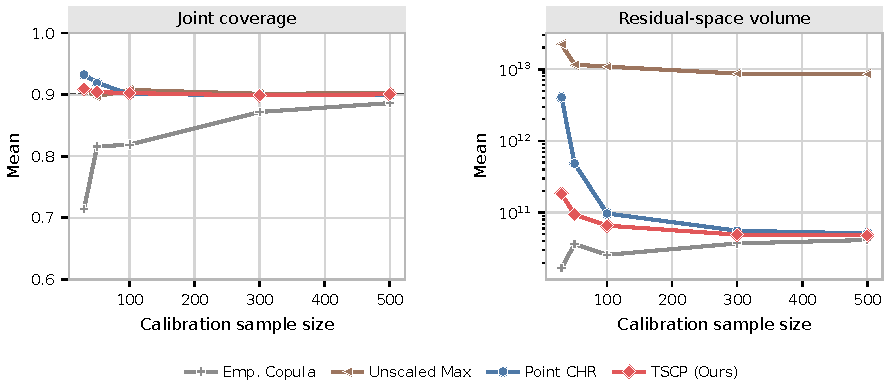
\includegraphics[width=0.9\textwidth]{figures/fig_body_abs_independent_gaussian.pdf}
\caption{Absolute-residual experiment with $d=10$, independent Gaussian
noise, and heterogeneous scales $(10,9,\ldots,1)$. Panels report mean joint
coverage and residual-space volume over 200 repetitions. The dashed line
marks the target coverage $0.9$. TSCP attains near-nominal coverage with
smaller residual-space volumes than Point CHR and Unscaled Max.}
\label{fig:gaussian-heter}
\end{figure}


Figure~\ref{fig:gaussian-homo} reports the corresponding homogeneous setting,
with $\epsilon_j\sim\mathcal{N}(0,1)$ for all $j\in[10]$. Unscaled Max is
the most efficient method with near-nominal coverage, while TSCP remains
competitive.
Together, these two settings show that coordinate adaptation is useful when
noise scales differ, whereas unscaled calibration can be more efficient
when a common scale is appropriate.

\begin{figure}[!htbp]
    \centering
    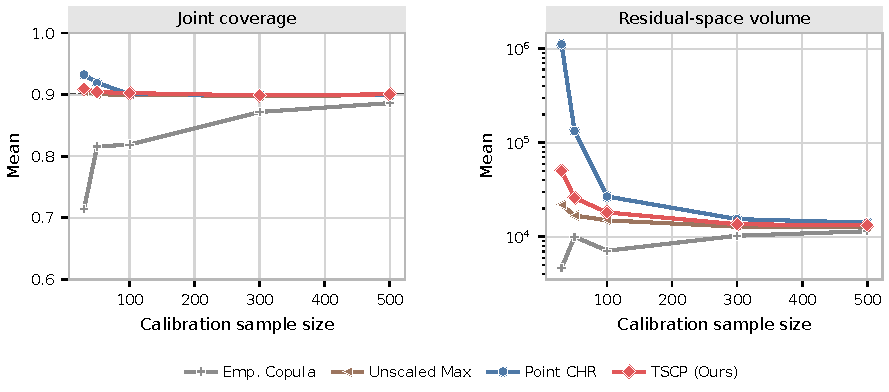
\includegraphics[width=0.9\textwidth]{figures/fig_body_abs_homogeneous_gaussian.pdf}
\caption{Absolute-residual experiment with $d=10$, independent Gaussian
noise, and unit scale in every coordinate. Panels report mean joint
coverage and residual-space volume over 200 repetitions. The dashed line
marks the target coverage $0.9$. Among methods with near-nominal coverage,
Unscaled Max has the smallest residual-space volume, while TSCP remains competitive.}
\label{fig:gaussian-homo}
\end{figure}

\subsubsection{Heterogeneous and Dependent Noise}

The dependent-noise experiment uses
$\boldsymbol{\epsilon}\sim\mathcal{N}(\boldsymbol{0},DRD)$, where
$D=\operatorname{diag}(10,9,\ldots,1)$ and $R$ is equicorrelated with
$\rho=0.6$. This simultaneously tests heterogeneous coordinate scales and
cross-output dependence. 

Figure~\ref{fig:body-abs-overview} reports joint
coverage, residual-space volume, and construction time. As in the independent
Gaussian setting with heterogeneous scales, TSCP attains near-nominal
coverage with smaller volumes than Point CHR and Unscaled Max.

\begin{figure*}[!htbp]
  \centering
  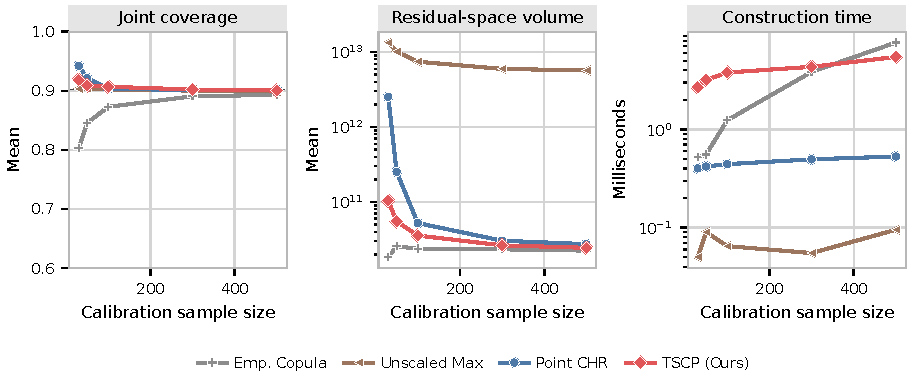
\includegraphics[width=0.94\textwidth]{figures/fig_body_abs_residual_overview.pdf}
  \caption{Absolute-residual experiment with $d=10$, heterogeneous Gaussian
  scales $(10,9,\ldots,1)$, and equicorrelation $\rho=0.6$. Panels report
  mean joint coverage, residual-space volume, and construction time over
  200 repetitions. The dashed line marks the target coverage $0.9$.
  Runtime excludes model fitting and residual computation.}
  \label{fig:body-abs-overview}
\end{figure*}

Figure~\ref{fig:body-abs-coordinate-bars} reports the coordinate-wise
interval lengths for all methods at $n=100$. The mean TSCP full interval length decreases
from $49.4$ on the noisiest coordinate to $5.0$ on the quietest coordinate.
In contrast, Unscaled Max assigns the same length, approximately $38.0$, to
every coordinate. Thus, similar overall coverage does not imply similar
coordinate-wise informativeness: TSCP allocates width according to coordinate scale
instead of allowing the noisiest output to determine all ten intervals. The
smaller Emp. Copula bars must be read together with its joint undercoverage in
Figure~\ref{fig:body-abs-overview}.

\begin{figure*}[t]
  \centering
  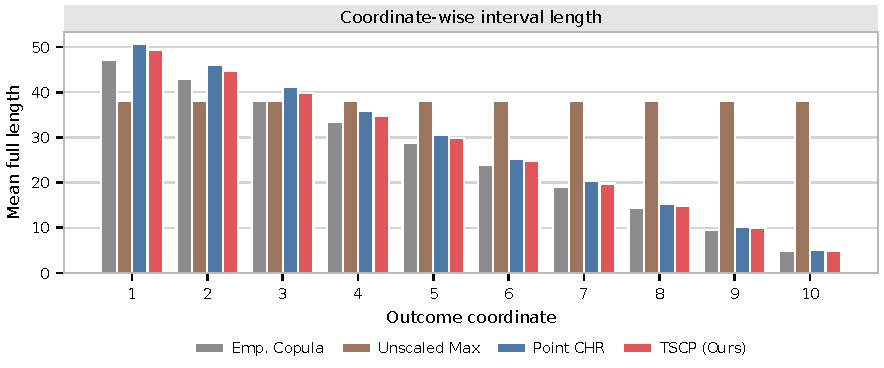
\includegraphics[width=0.90\textwidth]{figures/fig_body_abs_coordinate_bars.pdf}
  \caption{Coordinate-wise mean full interval lengths for the
  absolute-residual experiment with $d=10$, $n=100$, heterogeneous Gaussian
  scales $(10,9,\ldots,1)$, and equicorrelation $\rho=0.6$. Residual-space
  half-widths are multiplied by two to report full outcome intervals. Results
  average 200 independent repetitions. Unscaled Max assigns the same length to every coordinate, while others adapt to the coordinate scales.}
  \label{fig:body-abs-coordinate-bars}
\end{figure*}

\subsubsection{Partial Heteroskedasticity}
To distinguish heterogeneity across coordinates from heteroskedasticity with
respect to the input, we next make only the first five coordinates
heteroskedastic. For $j\leq5$, conditional on $X_1=x_1$, the noise standard
deviation is
\[
  \sigma_j(x_1)
  = (11-j)\sqrt{\frac{1+1.5x_1^2}{2.5}},
\]
while $\sigma_j(x_1)=11-j$ remains constant for $j>5$. The normalization preserves
$\mathbb{E}[\sigma_j^2(X_1)]=(11-j)^2$, so the comparison isolates
input-dependent variance and does not change the marginal second moments.
Figure~\ref{fig:body-partial-hetero} shows that TSCP remains close to the
target coverage $0.9$ across calibration sizes and continues to adapt coordinate-wise. This experiment does not
assert conditional coverage at each value of $X_1$.

\begin{figure*}[t]
  \centering
  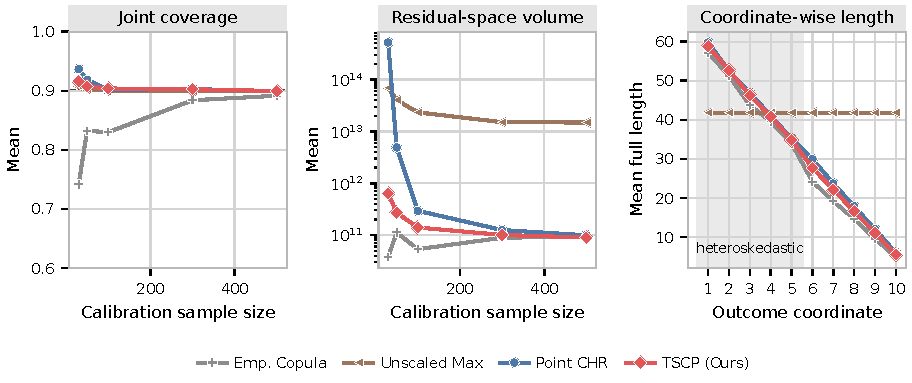
\includegraphics[width=0.94\textwidth]{figures/fig_body_partial_heteroskedasticity.pdf}
  \caption{Performance when only the first five of ten outcomes are
  heteroskedastic in $X_1$. The shaded coordinates in the right panel are the
  heteroskedastic ones; full interval lengths are shown for $n=100$.
  Results are averaged over 200 repetitions, and the dashed line marks
  the target joint coverage $0.9$.}
  \label{fig:body-partial-hetero}
\end{figure*}

\subsection{Quantile-Regression Residuals}
\label{sec:cqr-experiments}

We next replace absolute mean-regression residuals with coordinate-wise quantile regression residuals. Let $\widehat q_{\ell,j}(x)$ and $\widehat q_{u,j}(x)$ denote fitted
lower and upper conditional quantiles, ordered pointwise. The signed residual is
\[
  E_j(x,y)
  = \max\{\widehat q_{\ell,j}(x)-y_j,
           y_j-\widehat q_{u,j}(x)\}.
\]
Negative values correspond to observations strictly inside the base interval $[ \widehat q_{\ell,j}(x), \widehat q_{u,j}(x) ]$.
Because the TSCP theory is stated for nonnegative residuals, we use the
capped scores $\max\{E_j,0\}$. Capping prevents the calibrated interval from
shrinking the fitted base interval. We therefore use base-interval
miscoverage $0.5$ to limit the prevalence of negative signed scores.
This choice is not required by the method; Appendix~\ref{app:cqr-sensitivity}
examines other base-interval levels and a shifted-score transformation.
Capping can introduce ties at zero, but we can break them by adding a small random noise as a standard procedure in conformal inference.

Unscaled Max, CQHR, and Emp. Copula use the raw signed
residuals for fair comparison. CQHR uses the first
coordinate as reference and a numerical floor of $10^{-12}$ on base-interval
lengths when forming width ratios.

We use the same linear signal and ten-dimensional Gaussian features in~\eqref{eq:data-generator} with
$d=3$ Gaussian outcomes and independent noise scales $(3,2,1)$, fit separate
gradient-boosted quantile regressions using 2,400 training observations, and
evaluate on 600 test observations. Each quantile model uses 100 boosting
stages, maximum tree depth $5$, learning rate $0.05$, and minimum leaf size
$5$. The base-interval miscoverage is $0.5$ and
the final target miscoverage is $0.1$. Calibration sizes are
$n\in\{30,50,100,200\}$. Each of the 30 repetitions uses independently
generated training, test, and calibration samples.

Figure~\ref{fig:body-cqr} shows that
TSCP, CQHR, and Unscaled Max attain
near-nominal coverage, with TSCP producing the smallest mean outcome-space
volume among these three methods in the displayed settings. CQHR's volume
is sensitive to the fitted base interval, as examined in
Appendix~\ref{app:cqr-sensitivity}. Emp. Copula undercovers in this comparison.

\begin{figure*}[t]
  \centering
  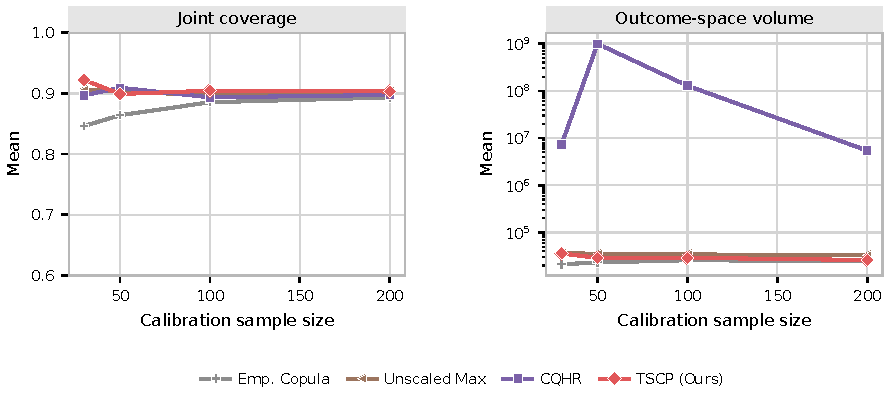
\includegraphics[width=0.88\textwidth]{figures/fig_body_cqr_comparison.pdf}
  \caption{CQR experiment with $d=3$ and base-interval miscoverage $0.5$.
  TSCP uses capped nonnegative scores, Unscaled Max, CQHR, and Emp. Copula use raw
  signed residuals. Results are averaged over 30 independent repetitions.}
  \label{fig:body-cqr}
\end{figure*}

Figure~\ref{fig:body-cqr-coordinate-bars} reports the corresponding
coordinate-wise comparison at $n=100$. In particular, TSCP preserves a substantially
shorter third-coordinate interval than Unscaled Max, while CQHR is much wider
on the second and third coordinates in this fitted-quantile design. As above,
the coordinate-wise lengths should be interpreted together with the joint
coverage panel rather than compared without regard to calibration.

\begin{figure*}[!htbp]
  \centering
  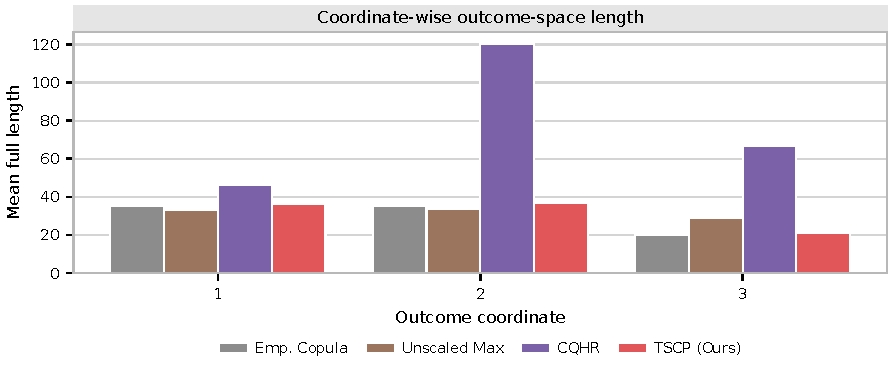
\includegraphics[width=0.82\textwidth]{figures/fig_body_cqr_coordinate_bars.pdf}
  \caption{Coordinate-wise mean full outcome-space lengths for the CQR
  experiment with $d=3$, $n=100$, base-interval miscoverage $0.5$, and final
  target coverage $0.9$. TSCP uses capped residuals, Unscaled Max and Emp. Copula
  use raw signed residuals, and CQHR uses its native construction. Results
  average 30 independent repetitions.}
  \label{fig:body-cqr-coordinate-bars}
\end{figure*}

\subsection{Real-Data Experiments}
\label{sec:real-data-experiments}

We evaluate six real-data benchmarks:
\texttt{rf2}~\citep{grigorios_tsoumakas_eleftherios_spyromitros-xioufis_william_groves_ioannis_vlahavas_2022},
\texttt{scm1d}~\citep{scm1d}, \texttt{scm20d}~\citep{scm20d},
\texttt{stock}~\citep{stock_portfolio_performance_390},
\texttt{student}~\citep{cortez2008student}, and
\texttt{energy}~\citep{tsanas2012energy}. Each result averages 200 random
training/calibration/test splits using proportions $75\%/5\%/20\%$. The
calibration sizes therefore range from $15$ on \texttt{stock} to $490$ on
\texttt{scm1d}. A multitask lasso with regularization parameter $10^{-4}$ is
used for \texttt{stock}; random forests are used for the other datasets. We use
absolute-residual scores and target coverage $0.9$ throughout. All methods
share the fitted model in each split. We report joint coverage,
residual-space volume, and construction time here; coordinate-wise
comparisons and search diagnostics appear in
Appendix~\ref{app:additional-real-experiments}.
Table~\ref{tab:real-data} reports coverage and residual-space volume for the
four primary methods.

\begin{table*}[!htbp]
\centering
\small
\begin{tabular}{llrrr}
\toprule
Dataset & Method & $d$ & Coverage & Volume \\
\midrule
\texttt{stock} & Unscaled Max & 6 & $0.940\,(0.057)$ & $6.03\mathrm{e}{-2}\,(1.57\mathrm{e}{-1})$ \\
 & Emp. Copula & 6 & $\color{red} 0.727\,(0.113)$ & $1.01\mathrm{e}{-5}\,(9.80\mathrm{e}{-6})$ \\
 & Point CHR & 6 & $1.000\,(0.000)$ & $\infty$ \\
 & \textbf{TSCP} & 6 & $0.956\,(0.059)$ & $\mathbf{1.86\mathrm{e}{-3}\,(8.55\mathrm{e}{-3})}$ \\
\addlinespace
\texttt{rf2} & Unscaled Max & 8 & $0.900\,(0.016)$ & $4.14\mathrm{e}{3}\,(2.90\mathrm{e}{3})$ \\
 & Emp. Copula & 8 & $\color{red}0.893\,(0.016)$ & $5.35\mathrm{e}{1}\,(4.69\mathrm{e}{1})$ \\
 & Point CHR & 8 & $0.901\,(0.022)$ & $\mathbf{6.85\mathrm{e}{1}\,(7.55\mathrm{e}{1})}$ \\
 & TSCP & 8 & $0.901\,(0.017)$ & $5.42\mathrm{e}{2}\,(1.50\mathrm{e}{3})$ \\
\addlinespace
\texttt{scm1d} & Unscaled Max & 16 & $0.900\,(0.016)$ & $2.74\mathrm{e}{39}\,(4.02\mathrm{e}{39})$ \\
 & Emp. Copula & 16 & $\color{red}0.893\,(0.016)$ & $1.09\mathrm{e}{39}\,(1.34\mathrm{e}{39})$ \\
 & Point CHR & 16 & $0.905\,(0.020)$ & $2.84\mathrm{e}{39}\,(5.43\mathrm{e}{39})$ \\
 & \textbf{TSCP} & 16 & $0.901\,(0.015)$ & $\mathbf{1.52\mathrm{e}{39}\,(2.61\mathrm{e}{39})}$ \\
\addlinespace
\texttt{scm20d} & Unscaled Max & 16 & $0.901\,(0.016)$ & $2.70\mathrm{e}{40}\,(2.92\mathrm{e}{40})$ \\
 & Emp. Copula & 16 & $\color{red}0.892\,(0.017)$ & $1.18\mathrm{e}{40}\,(1.19\mathrm{e}{40})$ \\
 & Point CHR & 16 & $0.902\,(0.023)$ & $3.00\mathrm{e}{40}\,(8.00\mathrm{e}{40})$ \\
 & \textbf{TSCP} & 16 & $0.901\,(0.016)$ & $\mathbf{1.53\mathrm{e}{40}\,(1.50\mathrm{e}{40})}$ \\
\addlinespace
\texttt{energy} & Unscaled Max & 2 & $0.917\,(0.049)$ & $1.58\mathrm{e}{1}\,(6.80\mathrm{e}{0})$ \\
 & Emp. Copula & 2 & ${\color{red}0.886\,(0.061)}$ & $5.41\mathrm{e}{0}\,(4.49\mathrm{e}{0})$ \\
 & Point CHR & 2 & $0.899\,(0.069)$ & $8.81\mathrm{e}{0}\,(2.42\mathrm{e}{1})$ \\
 & \textbf{TSCP} & 2 & $0.922\,(0.048)$ & $\mathbf{6.95\mathrm{e}{0}\,(4.43\mathrm{e}{0})}$ \\
\addlinespace
\texttt{student} & Unscaled Max & 3 & $0.904\,(0.055)$ & $\mathbf{1.51\mathrm{e}{2}\,(1.27\mathrm{e}{2})}$ \\
 & Emp. Copula & 3 & ${\color{red}0.861\,(0.073)}$ & $1.08\mathrm{e}{2}\,(7.19\mathrm{e}{1})$ \\
 & Point CHR & 3 & $0.939\,(0.057)$ & $6.89\mathrm{e}{2}\,(1.07\mathrm{e}{3})$ \\
 & TSCP & 3 & $0.912\,(0.056)$ & $1.98\mathrm{e}{2}\,(1.77\mathrm{e}{2})$ \\
\bottomrule
\end{tabular}
\caption{Performance on real datasets, averaged over 200 random splits. One
standard deviation is reported in parentheses. Bold volume denotes the
smallest average volume among TSCP, Point CHR, and Unscaled Max. Red coverage
values are more than two Monte Carlo standard errors below $0.9$, where the
standard error is the across-split standard deviation divided by $\sqrt{200}$.
This is a pointwise descriptive flag, not a simultaneous test or a proof of validity.
The calibration sizes are 15, 384,
490, 448, 38, and 32 in the order shown.}
\label{tab:real-data}
\end{table*}

Among TSCP, Point CHR, and Unscaled Max, TSCP has the smallest average
volume on \texttt{stock}, \texttt{scm1d}, \texttt{scm20d}, and
\texttt{energy}. Point CHR has the smallest volume on \texttt{rf2}, while
Unscaled Max has the smallest volume on \texttt{student}. Thus, the
coordinate-adaptive construction is beneficial in several datasets but is
not uniformly preferable. Emp. Copula produces smaller regions with
empirical coverage below the target.

Figure~\ref{fig:body-real-runtime} compares construction times.
TSCP constructs a region in $0.74$--$7.46$ milliseconds on
these datasets. It is slower than the algebraically simpler Unscaled Max and
Point CHR implementations, but substantially faster than Emp. Copula on the
two $16$-dimensional SCM datasets. 

The infinite Point CHR volume on \texttt{stock} should not be interpreted as
an intrinsic failure of the method. With only $n=15$ calibration observations,
its additional split leaves too few observations for a finite $0.9$ conformal
quantile. A practitioner committed to Point CHR would allocate a larger
fraction of the data to its final calibration stage, at the cost of fewer
observations for model and scale estimation.

\begin{figure*}[t]
  \centering
  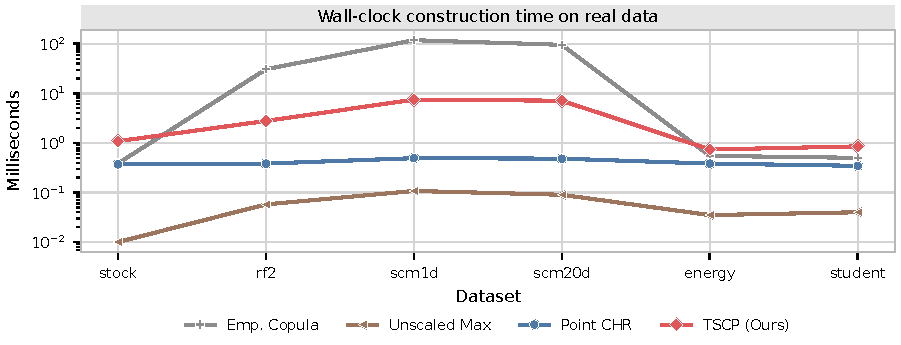
\includegraphics[width=0.90\textwidth]{figures/fig_body_real_runtime.pdf}
  \caption{Average wall-clock time for conformal region construction on the
  six real datasets. The vertical axis is logarithmic and reports
  milliseconds. All methods use the same fitted regression model in each
  split; model fitting and residual computation are excluded.}
  \label{fig:body-real-runtime}
\end{figure*}




\subsubsection{Interpretability of Rectangular Prediction Sets}
To emphasize their interpretability, Table~\ref{tab:toy} displays the rectangular prediction sets produced by different methods for two representative test points from the \emph{energy} dataset, where $d=2$. In this setting, rectangular prediction sets consist of pairs of simultaneous prediction intervals that aim to jointly contain the true outcomes with probability $90\%$.

\begin{table}[!htbp]
\centering
\captionsetup[subtable]{justification=centering}
\small
\begin{subtable}{\linewidth}
\centering
\begin{tabular}[t]{l c c c c}
\toprule
\textbf{Test 1/Methods} 
& Outcome 1 & Outcome 2 & Volume & Ground Truth \\
\midrule
Unscaled Max & [31.70, 38.94] & \textbf{[34.74, 41.98]} & 13.09 & \multirow{4}{*}{(35.40, 39.22)} \\
Emp. copula & \textbf{[34.36, 36.28]} & \textbf{[34.74, 41.98]} & {3.47} &\\
Point CHR & [34.29, 36.36] & [31.45, 45.27] & 7.14 &\\
TSCP & [34.28, 36.36] & [33.63, 43.08] & 4.93 &\\
\midrule
\end{tabular}
\end{subtable}

\small
\begin{subtable}{\linewidth}
\centering
\begin{tabular}[t]{l c c c c}
\midrule
\textbf{Test 2/Methods} 
& Outcome 1 & Outcome 2 & Volume & Ground Truth \\
\midrule
Unscaled Max & [25.44, 32.67] & \color{red}[29.34, 36.58] & 13.09 & \multirow{4}{*}{(29.88, 28.31)} \\
Emp. copula & \textbf{[28.10, 30.02]} & \color{red}[29.34, 36.58] & 3.47 & \\
Point CHR & [28.02, 30.09] & [26.05, 39.87] & 7.14 & \\
TSCP & [28.01, 30.10] & \textbf{[28.24, 37.69]} & {4.93} & \\
\bottomrule
\end{tabular}
\end{subtable}

\caption{Illustration of rectangular conformal prediction sets for two test
points from the \emph{energy} dataset. Volumes are computed in residual
space. Intervals that fail to cover the corresponding true outcomes are
highlighted in \textcolor{red}{red}; the shortest interval containing each
true outcome is highlighted in \textbf{bold}. This example is illustrative:
conformal coverage guarantees hold on average, not for individual test points.}
\label{tab:toy}
\end{table}

\endgroup


\section{Discussion and Future Work}
\label{sec:discussion}

The core idea underlying the method presented in this paper is the explicit standardization of residuals, which contributes both to the transparency and to the computational efficiency of the resulting prediction sets. As with other standardization-based methods, however, this strategy introduces some sensitivity to outliers. This behavior is visible in the numerical experiments based on the \emph{rf2} dataset, where a small number of influential observations can substantially expand the resulting prediction sets. The contamination study in Appendix~\ref{app:contamination} likewise distinguishes stable empirical coverage from substantial volume inflation. An important direction for future work is therefore the development of robust extensions of our method, for example through rescaling based on median absolute deviation or quantile-based normalizations, while preserving the exchangeability required for conformal validity.

Another direction is a direct treatment of signed residuals without capping or an additive shift. The CQR comparisons in Section~\ref{sec:cqr-experiments} and Appendix~\ref{app:cqr-sensitivity} illustrate the limitations of these transformations. A direct extension could enable shrinkage of baseline prediction sets when starting from quantile regression models that already exhibit conservative coverage. It would also be of interest to adapt the proposed approach to settings with non-numerical outcomes, such as categorical or ordinal responses. Finally, our method could be extended to handle partly observed outcomes \citep{braun2025multivariate}.

\section*{Software Availability}

A software implementation of the methods described in this paper, along with code necessary to reproduce the numerical experiments, is available online at \url{https://github.com/OTheMagic/multi-target-scaling.git}.

\acks{The authors thank Rundong Ding and Dr.~Yizhe Zhu for helpful suggestions during an oral presentation of an earlier version of this work. M.S.~was partly supported by NSF grant DMS 2210637, a USC-Capital One CREDIF award, and a Google Research Scholar award.}


%%% Local Variables:
%%% mode: latex
%%% TeX-master: "main"
%%% End:
